\documentclass[12pt,a4paper]{article}
%----------------------------------------
% German language
% \usepackage[ngerman]{babel}
%----------------------------------------
% Input in UTF8 accepted
\usepackage[utf8]{inputenc}
%----------------------------------------
% Math-packages
\usepackage{mathtools}
\usepackage{amsmath}
\usepackage{amssymb}
%----------------------------------------
% Design choices (?)
%\usepackage{scrlayer-scrpage}
%\pagestyle{scrheadings}
% \clearscrheadfoot
%----------------------------------------
% Footnotes in tables
\usepackage{tablefootnote}
%----------------------------------------
%----------------------------------------
% no parindent
\usepackage{parskip}
\setlength{\parindent}{0em}
%----------------------------------------
% different gap between paragraphs
\setlength{\parskip}{1.3ex}
%----------------------------------------
% spacing between lines
\usepackage[onehalfspacing]{setspace}
%----------------------------------------
% Hurenkinder und Schusterjungen vermeiden
\clubpenalty = 10000
\widowpenalty = 10000
\displaywidowpenalty = 10000
%----------------------------------------
% Geometry package
\usepackage{geometry}
\geometry{
	paper=a4paper, % Change to letterpaper for US letter
	top=3cm, % Top margin
	bottom=3cm, % Bottom margin
	left=3cm, % Left margin
	right=3cm, % Right margin
	%showframe, % Uncomment to show how the type block is set on the page
}
%----------------------------------------
% References
\usepackage[backend=biber, maxbibnames=99, sortcites=true]{biblatex}
\addbibresource{references.bib}
%----------------------------------------
\usepackage{graphicx}
\graphicspath{ {./assets/images/} }
%----------------------------------------
\usepackage[nottoc]{tocbibind}
%----------------------------------------
\usepackage[onehalfspacing]{setspace}
%----------------------------------------
% formats text "better"
\usepackage{microtype}
%----------------------------------------
% "better" tables
\usepackage{booktabs}
\usepackage{tabularx}
\usepackage{multirow}
\usepackage{makecell}
% for big tables
\usepackage{adjustbox}
%----------------------------------------
%Colours:
\usepackage[dvipsnames, table]{xcolor}
%----------------------------------------
% Definition Box
\usepackage[framemethod=TikZ]{mdframed}
\mdfdefinestyle{enviStyle}{
	innertopmargin = 10pt,
	linewidth      = 1pt,
	frametitlerule = true,
	roundcorner    = 2pt%
}
\usepackage{sectsty}
\newenvironment{CountingDefinition}[2][]{%
	\vspace*{1.7ex}
	\ifstrempty{#1}%
	{\mdfsetup{%
			frametitle={{\strut ~}}}
	}%
	{\mdfsetup{%
			frametitle={{\strut ~#1}}}%
	}%
	\mdfsetup{
		nobreak                   = true,
		linecolor                 = RedViolet,
		frametitlebackgroundcolor = RedViolet!50,
		style                     = enviStyle
	}
	\begin{mdframed}[]\relax%
		\label{#2}}{\end{mdframed}}
	%----------------------------------------
% Design
%\sectionfont{\color{RedViolet}}
%\subsectionfont{\color{RedViolet}}
\renewcommand{\labelitemi}{$\textcolor{RedViolet}{\bullet}$}
\renewcommand{\labelitemii}{$\textcolor{RedViolet}{\circ}$}
\renewcommand{\labelitemiii}{$\textcolor{RedViolet}{\diamond}$}
\renewcommand{\labelitemiv}{$\textcolor{RedViolet}{\ast}$}
%----------------------------------------
% Position figures, etc.
\usepackage{float}
%----------------------------------------
% Lines and dotted lines and other designs
\usepackage{dashrule}
\usepackage{tikz}
\usepackage{tikzpagenodes}
%----------------------------------------
%----------------------------------------
% Hyperref package
\usepackage{hyperref}
\hypersetup{
	colorlinks=true,
	linkcolor=black,
	filecolor=black,      
	urlcolor=RedViolet,
	citecolor=black
}
% To include the README files:
%\usepackage{markdown}
%----------------------------------------
% Linebreaks in \texttt:
\usepackage[htt]{hyphenat}
%----------------------------------------
% Footnote citations with \myfootcite
\DeclareBibliographyCategory{skipbibliography}

\DeclareCiteCommand{\myfootcite}[\mkbibfootnote]
	{\usebibmacro{prenote}}
	{\addtocategory{skipbibliography}{\thefield{entrykey}}%
		\usedriver
			{\DeclareNameAlias{sortname}{default}}
			{\thefield{entrytype}}}
		{\multicitedelim}
		{\usebibmacro{postnote}}
%----------------------------------------
% Rounded corners in graphics with \cutpic
\newsavebox{\picbox}	
\newcommand{\cutpic}[3]{
	\savebox{\picbox}{\includegraphics[width=#2]{#3}}
	\tikz\node [draw, rounded corners=#1, line width=4pt,
	color=white, minimum width=\wd\picbox,
	minimum height=\ht\picbox, path picture={
		\node at (path picture bounding box.center) {
			\usebox{\picbox}};
	}] {};}

%----------------------------------------------------------------------------
%----------------------------------------------------------------------------

\begin{document}
	
\pagenumbering{roman}


\begin{titlepage}	
	\begin{center}
	\centering
	\vspace*{-4em}
	\begin{tabularx}{\linewidth}{@{}lXr@{}}
		\makecell{
\includegraphics[height=1.5cm]{umu.png}}
		& &\makecell{
\includegraphics[height=0.7cm]{codemill.png}}\\
	\end{tabularx}\\%
	\vfill
	{\scshape\LARGE Ume\aa \  University \par}
	and \par 
	\vspace*{-0.8em}
	{\scshape\LARGE Codemill \par}
	\vspace{1cm}
	{\scshape\Large Master Thesis \par }
	\vspace{1.5cm}
	{\huge\bfseries Multimedia Processing: Exploring Real-Time Colour Correction and Grading with JIT \par}
	\vspace{2cm}
	{\Large Pina Kolling\par}
	% \texttt{ens21pkg@cs.umu.se} \par
	\vfill
	Supervised by\par
	Dr. Cem \textsc{Okulmus} \par 
	and \par 
	Urban \textsc{Söderberg} 
	
	\vfill
	
	% Bottom of the page
	{\large \today \par}
\end{center}
\end{titlepage}

%---------------------------------------------------------------------------------------------------



{\color{RedViolet} \rule{\textwidth}{1pt}}

{\color{RedViolet}\dotfill}

\begin{abstract}
	\noindent Lorem ipsum dolor sit amet, consetetur sadipscing elitr, sed diam nonumy eirmod tempor invidunt ut labore et dolore magna aliquyam erat, sed diam voluptua. At vero eos et accusam et justo duo dolores et ea rebum. Stet clita kasd gubergren, no sea takimata sanctus est Lorem ipsum dolor sit amet. Lorem ipsum dolor sit amet, consetetur sadipscing elitr, sed diam nonumy eirmod tempor invidunt ut labore et dolore magna aliquyam erat, sed diam voluptua. At vero eos et accusam et justo duo dolores et ea rebum. Stet clita kasd gubergren, no sea takimata sanctus est Lorem ipsum dolor sit amet. TODO
\end{abstract}
{\color{RedViolet}\dotfill}

{\color{RedViolet} \rule{\textwidth}{1pt}}

%---------------------------------------------------------------------------------------------------

\newpage


\setcounter{page}{1}

%\setstretch{0.6}

\newgeometry{
	top=2cm, % Top margin
	left=3cm, % Left margin
	right=3cm, % Right margin
	bottom = 2cm
}

\begin{spacing}{0.95}
		
	\tableofcontents
	
\end{spacing}

\newgeometry{
	top=3cm, % Top margin
	left=3cm, % Left margin
	right=3cm, % Right margin
	bottom = 3cm
}


%\setstretch{1.5}



\newpage

\pagenumbering{arabic}

\setcounter{page}{1} 
%

%
%
%
%
%=======================================================================================================
%
%
%
%
%=======================================================================================================
% CHAPTER: INTRODUCTION
%=======================================================================================================
\newpage
\section{Introduction} \label{section:introduction}


The popularity of streaming is growing, with an increasing number of people using online streaming platforms for their entertainment and approximately 1.8 billion subscriptions to video streaming services. \myfootcite{nielsen}\textsuperscript{,} \myfootcite{stats}
%
With this increased popularity, the demand for user-driven real-time visual customization in the web browser for streamed videos has also increased.


















%-------------------------------------------------------------------------------------------------------
\subsection{Motivation} \label{subsection:motivation}


The colouring of a video can evoke different emotions and set an overall tone to the perception of the content. For instance, cool colours like blue can convey cold weather, while warm colours like yellow can create a feeling of warmth and sunlight. 
The colouring of a video is a powerful tool that can significantly impact the conveyed mood and atmosphere.\myfootcite{colorgrading1}\textsuperscript{,} \myfootcite{colorgrading2}




\begin{figure}[H]
	\begin{center}
		\cutpic{0.3cm}{0.3\textwidth}{2_blau.jpg}
		%\hspace*{0.01\textwidth}
		\cutpic{0.3cm}{0.3\textwidth}{2.jpg}
		%\hspace*{0.01\textwidth}
		\cutpic{0.3cm}{0.3\textwidth}{2_gelb.jpg}
		\label{figure:coloursblueandyellow}
		\caption[Photo in different colour tones]{The original photo can be seen in the middle, while the picture on the left has more blue tones and the picture on the right more yellow tones.}
	\end{center}
\end{figure}
%
%
%
The use-cases for on-the-fly adjustments of the video colour arise from different reasons. 
One of them is that each screen, ranging from computer monitors, TVs, smartphones and tablets to beamers, has unique characteristics that can influence the perceived colour palette. 
In addition to this, the light conditions can influence the appearance of the colours.
With real-time colour corrections, the user can adjust the colour and cancel out variations that are caused by the device or environment to have a consistent experience.

Real-time colour correction is a solution that not only addresses the variability in device displays but also enables users to adjust the image according to their preferences.

Additionally, users with visual problems or specific colour perception might benefit from real-time colour correction to enhance the visibility and distinction of the on-screen elements. 




%1. **Device Variability:** As mentioned earlier, different devices have distinct display characteristics. Users may prefer to adjust colours to compensate for variations in brightness, contrast, or colour rendering among devices.

%2. **Personal Preferences:** Everyone perceives colours differently, and personal preferences for visual aesthetics vary. Real-time colour correction empowers users to customize the viewing experience according to their individual tastes.

%3. **Environmental Conditions:** Lighting conditions in the viewing environment can impact how colours appear on the screen. Real-time colour correction allows users to adapt to different lighting situations, ensuring optimal visibility and comfort.

%4. **Accessibility Considerations:** Users with visual impairments or specific color perception needs may benefit from real-time colour correction to enhance visibility and distinguishability of on-screen elements.


%6. **Cultural Differences:** Cultural preferences and associations with colours can vary globally. Real-time colour correction accommodates diverse cultural perspectives, allowing users to align the visual presentation with their cultural preferences.













%-------------------------------------------------------------------------------------------------------
\subsection{Research Questions} \label{subsection:research% Formulate specific research questions that your thesis aims to answer.
	TODOquestions}


This thesis revolves around the implementation of video colour correction using Just-In-Time (JIT) techniques. 	
JIT is used for on-the-fly conversion of video files and optimizing them for streaming. 
%This process includes the transformation of a video file, potentially one with non-web-friendly formats, into a more suitable format for the playback in web browsers.
The demand for efficient and dynamic video processing tools is increasing and with this, the ability to perform on-the-fly colour correction becomes increasingly valuable. 

The goal of this thesis is to explore the feasibility of implementing the video grading process with JIT, with the focus on real-time colour correction and to implement such a solution, if possible. This project lies in the area of multimedia processing, video editing and real-time computing and is done in cooperation with the company Codemill, that is introduced in Section \ref{subsection:codemill}.


%The infrastructure of the system is visualized and explained in Chapter~\ref{section:designandimplementation}.

The project aims to address the feasibility (and potentially effectiveness) of implementing video colour correction using JIT in the context of real-time video streaming. The following question is relevant:

\begin{itemize}
	\item Is it possible to obtain colour-corrected video results on the fly, meaning in real-time, using JIT?
\end{itemize}

After answering this research question, the following questions might occur and be put into perspective:

\begin{itemize}
	\item Are there multiple solutions for implementing video colour correction, and if so, how do they compare in terms of performance, accuracy, and efficiency?
	\item How does the possibility of video colour correction expand potential applications of JIT in the domain of multimedia processing?
	\item What is the usability and performance of the proposed solution in real-world scenarios, regarding real-time video colour correction?
\end{itemize}

The aim is to contribute insights into the technological and scientific aspects of real-time video processing, exploring the possibilities and potential applications introduced by using JIT to implement colour grading. 







%-------------------------------------------------------------------------------------------------------
\subsection{Codemill} \label{subsection:codemill}
% Provide context, highlight the problem space, and explain the motivation behind the project.

Codemill was founded in 2008 in Ume\aa \ (Sweden).\myfootcite{codemill_now}\textsuperscript{,} \myfootcite{codemill_old}\textsuperscript{,} \myfootcite{codemill_linkedin}
As of February 2024, they employ over 60 employees. \myfootcite{codemill} 
Codemill is an IT-Consulting company that focussed on the production and distribution of broadcast media. Their Accurate Video Player that is described in Section~\ref{subsection:accuratevideo}, is part of this thesis and a cloud native software that is being used by the world's leading studios, broadcasters and media service providers. \myfootcite{codemill_linkedin}\textsuperscript{,}  \myfootcite{codemill_avp}
The infrastructure of the system that this thesis evolves around is visualized and explained in Chapter~\ref{section:designandimplementation}.












%-------------------------------------------------------------------------------------------------------
\subsection{Related Work} \label{subsection:relatedwork}










%-------------------------------------------------------------------------------------------------------
\subsection{Structure} \label{subsection:structure}
% Outline the structure of the thesis, briefly describing each chapter's content.









%
%
%
%
%=======================================================================================================
%
%
%
%
%=======================================================================================================
% CHAPTER: Preliminaries
%=======================================================================================================
\newpage
% \section{Preliminaries} \label{section:preliminaries}

\section{Theoretical Foundation of Colour} \label{subsection:theoreticalfoundationofcolour}

In this chapter, the terms colour correction and colour grading are explained and colour theory is introduced. 
In addition to this, the effects of different colours in media and their association are explained.





%-------------------------------------------------------------------------------------------------------
\subsection{Colour Correction and Colour Grading} 


Colour correction and colour grading are both processes used in film making, photography, and digital art to adjust and enhance the colour of images or videos. 

While they are related, they serve different purposes and are typically performed at different stages of production.

Colour correction aims to correct technical imperfections and achieve a natural-looking image, while colour grading focuses on enhancing the visual aesthetics and storytelling aspects.~\cite{cc_cg_1, cc_cg_2}


Colour correction is the process of adjusting the overall colour balance, contrast, and exposure of an image or video to achieve a more accurate representation of the scene as it was captured by the camera. It involves correcting potential technical issues such as white balance, exposure inconsistencies, and colour inaccuracies caused by the camera or lighting conditions.~\cite{cc1, cc_cg_1, cc_cg_2}

This is typically done in the early stages of post-production to ensure that the footage looks natural and consistent across different shots and scenes.~\cite{cc1}


Colour grading, on the other hand, is the creative process of altering the colour and mood of an image or video to evoke a specific aesthetic or emotional response. The effects of different colours are described in Section~\ref{subsection:effectsofdifferentcolours}.
Colour grading involves making stylistic choices to enhance the visual storytelling or the overall cinematic look of the footage. It can involve manipulating individual colours, adjusting contrast, saturation, and applying various other colour grading techniques.~\cite{cc_cg_1, cc_cg_2}

Colour grading is often performed after colour correction and is considered a more artistic and subjective process. It allows film makers and photographers to establish a unique visual style and enhance the narrative impact of their work.~\cite{cc_cg_1, cc_cg_2}


In summary, colour correction and colour grading serve different purposes and are performed at different stages of post-production. Colour correction ensures technical accuracy and consistency, while colour grading adds artistic flair and enhances visual storytelling.~\cite{cc1, cc_cg_1, cc_cg_2}








%-------------------------------------------------------------------------------------------------------
% \subsection{Colour Theory}










\newpage
%-------------------------------------------------------------------------------------------------------
\subsection{Effects of different colours} 
\label{subsection:effectsofdifferentcolours}

Different colours can convey a different understanding of a scene to the viewer or even influence the viewers emotions. 
The different colours have distinct psychological associations, which influences how viewers perceive and interpret the content.~\cite{colour}
%But it needs to be considered that colours can carry cultural and contextual meanings that can vary across different societies and individuals. 


In different visual media, including art, photos, or videos, the strategic use of colour can effectively communicate themes, evoke emotions, and guide viewer interpretation.~\cite{cc_cg_1, cc_cg_2, colour}


In the following, different colours with their psychological associations are listed and example pictures are shown.



%-------------------------------------------------------------------------
%\subsubsection{Red}
\textbf{\textcolor{Maroon}{Red}}

%
%

\begin{minipage}{0.5\textwidth}
	\begin{figure}[H]
		\begin{center}
			\cutpic{0.3cm}{\textwidth}{fliegenpilz.jpg}
			\label{figure:red}
			\caption[Picture of a Amanita muscaria in Sweden with alarming red colour.]{Picture of a Amanita muscaria in Sweden with alarming red colour.}
		\end{center}
	\end{figure} \hfill
\end{minipage}\begin{minipage}{0.05\textwidth}
	\ 
\end{minipage}\begin{minipage}{0.45\textwidth}
	The colour red is often associated with intense emotions such as passion, excitement, and danger. Viewing it on self or others has even been shown to increase the perception of aggressiveness and dominance.~\cite{red_dominance} Wearing the colour in sport competitions and events red has been shown to enhance performance and the perceived performance.~\cite{colour, red_sport}
	
	In visual media, the use of red can evoke feelings of urgency, power, and love. For example a video with flashes of red light may create a feeling of tension or alarm while a female wearing red can increase the perceived attraction.~\cite{colour, red_romance}
	
	Beyond its symbolism in human emotions and cultural contexts, red also serves as a prominent warning colour in nature. One example of this is the

\end{minipage}

\vspace*{-1.2em}
toxic fly agaric mushroom (Amanita muscaria), which can be seen in Figure \ref{figure:red}.
The instinctual reaction to red is used in various contexts, including traffic signals and emergency exits, where the color serves as a clear and universally understood signal.







\newpage
%-------------------------------------------------------------------------
%\subsection{Blue} 
\textbf{\textcolor{BlueViolet}{Blue}}

%
\begin{minipage}{0.45\textwidth}
	The colour blue is often linked to feelings of calmness and stability. In videos and pictures, the presence of blue tones can create a sense of relaxation. For instance, the photo in Figure \ref{figure:blue} of a lake scene in Sweden with shades of blue in the water and the sky can evoke a peaceful mood.
	
	For instance, blue stores and logos have been shown to increase the perception of expected quality and trustworthiness.~\cite{blue_trust}
	
	But this is not the only association with the colour blue. While it might
	
	

\end{minipage}\begin{minipage}{0.05\textwidth}
\ 
\end{minipage}\begin{minipage}{0.5\textwidth}
\begin{figure}[H]
	\begin{center}
		\cutpic{0.3cm}{\textwidth}{lake.jpg}
		\label{figure:blue}
		\caption[Picture of a lake in Sweden with mainly blue tones.]{Picture of a lake in Sweden with mainly blue tones.}
	\end{center}
\end{figure}\hfill
\end{minipage}

\vspace*{-1.2em}
 evoke feelings of calmness or trustworthiness in certain contexts, it can also represent sadness or coldness depending on the situation.


%-------------------------------------------------------------------------
%\subsection{Green}
\textbf{\textcolor{ForestGreen}{Green}}

%
%
\begin{minipage}{0.5\textwidth}
		\begin{figure}[H]
		\begin{center}
			\cutpic{0.3cm}{\textwidth}{forest.jpg}
			\label{figure:green}
			\caption[Picture of a forest in Sweden with mainly green tones.]{Picture of a forest in Sweden with mainly green tones.}
		\end{center}
	\end{figure}\hfill
\end{minipage}\begin{minipage}{0.05\textwidth}
	\ 
\end{minipage}\begin{minipage}{0.45\textwidth}
	Green is associated with nature, growth, and harmony. In visual media, the use of green can symbolize renewal, freshness, and balance. For example, the picture in Figure \ref{figure:green} of a forest in Sweden can evoke feelings of vitality  and  may convey a sense of natural beauty and harmony.
	
	TODO references
	
	TODO more text
	
	TODO more text
\end{minipage}


%-------------------------------------------------------------------------
%\subsection{Yellow}
\textbf{\textcolor{YellowOrange}{Yellow}}

%
%
\begin{minipage}{0.45\textwidth}
	Yellow is often associated with happiness, optimism, and energy. When used in videos or pictures, yellow can evoke feelings of warmth, cheerfulness, and positivity. For instance, a photograph capturing a bright yellow sunrise as seen in Figure \ref{figure:yellow} can convey a sense of warmth, hope and optimism.
	
	TODO references
	
	TODO more text
	
	TODO more text
	
\end{minipage}\begin{minipage}{0.05\textwidth}
	\ 
\end{minipage}\begin{minipage}{0.5\textwidth}
	\begin{figure}[H]
		\begin{center}
			\cutpic{0.3cm}{\textwidth}{sunset.jpg}
			\label{figure:yellow}
			\caption[Picture of a sunrise in Sweden with mainly yellow tones.]{Picture of a sunrise in Sweden with mainly yellow tones.}
		\end{center}
	\end{figure}\hfill
\end{minipage}







%-------------------------------------------------------------------------
%\subsection{Black and White}

\textbf{\textcolor{gray}{Black and white}}


\begin{minipage}{0.5\textwidth}
	TODO picture Umea bridge in black and white
\end{minipage}\begin{minipage}{0.05\textwidth}
	\ 
\end{minipage}\begin{minipage}{0.45\textwidth}
	Black and white or greyscales are often used to evoke a sense of timelessness or simplicity. In visual media, the absence of colour can draw attention to shapes, textures, and contrasts. For example, a black and white photograph of a city skyline can emphasize the architectural details and create a dramatic atmosphere or, depending on the context, it may evoke a sense of nostalgia.
	
	TODO more text
	
	TODO more text
	
\end{minipage}

%

%\section{Conclusion}

%The emotional impact of colors in videos and pictures cannot be overstated. By understanding the psychological associations of different colors, creators can effectively convey emotions, set the mood, and engage viewers on a deeper level. Whether it's the passionate reds, calming blues, or vibrant yellows, each color has the power to evoke a unique emotional response, enriching the visual experience for the audience.


%Picture ideas:    

%Red: A picture of a sunset with rich red hues, or a close-up shot of a red rose.

%Blue: Capture an image of a tranquil lake with blue reflections, or a serene sky with fluffy clouds.

%Green: Take a photograph of a lush forest with vibrant green foliage, or a close-up of fresh grass after rainfall.

%Yellow: Capture the golden glow of a sunrise or sunset, or photograph a field of sunflowers bathed in sunlight.

%Black and White: Photograph a classic cityscape with stark contrasts between buildings and shadows, or capture the simplicity of a monochrome portrait.








%---------------------------------------------------------------------------
\newpage
%---------------------------------------------------------------------------

\section{Technical Background} \label{subsection:technicalbackground}

%-------------------------------------------------------------------------------------------------------
\subsubsection*{Video Transcoding} 

Transcoding is the conversion of one digital data format into another.~\cite{transcoding}







%-------------------------------------------------------------------------------------------------------
\subsubsection*{Video Compression with h.264} 
% Explain WebRTC

\begin{CountingDefinition}[h.264]{def:h264}
	
	h.264 refers to a video compression standard. In the context of real-time communication, h.264 is one of the video codecs that can be used to compress and decompress video streams.
	
\end{CountingDefinition}







%-------------------------------------------------------------------------------------------------------
\subsubsection*{WebRTC} 
% Explain WebRTC

\begin{CountingDefinition}[WebRTC]{def:WebRTC}
	
	Web Real-Time Communication (WebRTC), is a free, open-source project that provides web browsers and mobile applications with real-time communication. It enables direct communication between browsers or applications, allowing for peer-to-peer communication without the need for intermediary servers in certain scenarios.
	
\end{CountingDefinition}

WebRTC supports various video codecs, and h.264 is popular due to its efficiency in compressing video data while maintaining good quality. It is widely used for video conferencing, streaming, and other real-time communication applications. The video streams exchanged between the browser and the backend are encoded and decoded using h.264.






%-------------------------------------------------------------------------------------------------------
\subsubsection*{Audio Video Interleave} 

Audio Video Interleave (AVI) is a file format that can contain audio and video information to allow synchronized playback of audio and video components. 
It is a container format, which means that it can contain multiple streams of audio and video data, along with other multimedia data such as subtitles.~\cite{avi}












%-------------------------------------------------------------------------------------------------------
\subsubsection*{Named Pipe} 

A named pipe is a type of interprocess communication (IPC) mechanism. It provides a way for processes to pass data to each other and it is bidirectional. 
Named pipes follow a First-In-First-Out (FIFO) structure: The first data written into the pipe is the first data to be read. This maintains a sequential order for data transmission.
A traditional pipe is \textit{unnamed} and terminates when its process terminates. A named pipe can last beyond the life of the process, as long as the system is running.~\cite{namedpipe}









%-------------------------------------------------------------------------------------------------------
\subsubsection*{REST} 


Representational State Transfer (REST) is an architectural style for designing networked applications. A REST Application Programming Interface (API) exposes a set of endpoints (URLs) that allow communication between different software systems over the internet and it uses the hypertext transfer protocol (HTTP) methods.~\cite{IEEE_Rest, webservice, Nodejs_Rest}











%-------------------------------------------------------------------------------------------------------
\subsubsection*{JIT} 
%
\begin{CountingDefinition}[JIT]{def:JIT}
	
	JIT (Just-In-Time), in the context of video files for streaming, refers to a dynamic software solution employed for real-time video transformation on a server. It is used for on-the-fly conversion of video files, optimizing them for streaming. The process includes the transformation of a video file, potentially one with non-web-friendly formats, into a more suitable format for the playback in web browsers.
	
\end{CountingDefinition}









%
%
%
%
%=======================================================================================================
%
%
%
%
%=======================================================================================================
% CHAPTER: SYSTEM REQUIREMENTS AND SPECIFICATIONS
%=======================================================================================================
\newpage
\section{System Requirements and Specifications} \label{section:systemrequirementsandspecifications}

%Define the overall goals and objectives of your project.
%Specify the functional and non-functional requirements of the system. This includes what the system is expected to do, its features, and any constraints it must adhere to.
%Outline any specific hardware or software requirements necessary for the project.
%Detail the methodologies or approaches you'll use for system development.



%-------------------------------------------------------------------------------------------------------
\subsection{User Requirements} \label{subsection:userrequirements}
% Identify and describe the requirements from the end-user perspective.


%-------------------------------------------------------------------------------------------------------
\subsection{Technical Requirements} \label{subsection:technicalrequirements}
% Detail the technical requirements for the system.

Seems not to run on Windows.





%
%
%
%
%=======================================================================================================
%
%
%
%
%=======================================================================================================
% CHAPTER: DESIGN AND IMPLEMENTATION
%=======================================================================================================
\newpage
\section{Design and Implementation} \label{section:designandimplementation}







%-------------------------------------------------------------------------------------------------------
\subsection{Architecture Design} \label{subsection:architecturedesign}
% Describe the overall architecture of the system.

%Provide an overview of the system architecture and design. This could include high-level diagrams, such as system flowcharts or architecture diagrams, to illustrate the structure of the software.
%Introduce the existing codebase and its components. Briefly describe the major modules or sections of the code.
%Explain the design decisions made during the development process. Discuss the rationale behind the chosen architecture, programming languages, and frameworks.
%Present any relevant design patterns or paradigms applied in the codebase.
%Provide a detailed description of how the existing code works. This involves explaining the functionality of key modules or sections, the flow of data, and how different components interact.
%If applicable, discuss any algorithms or data structures implemented in the codebase.
%Highlight any challenges or considerations encountered during the implementation phase and how they were addressed.
%Include code snippets, illustrations, or diagrams to enhance the understanding of your codebase.

TODO: Short overview/introduction of architecture and explain structure of this section?





The connection from the Python backend to the Melt framework can use Melt's capabilities for video editing, processing, transcoding, rendering or playback. The system includes real-time communication via WebRTC, where Melt is involved in handling and manipulating video content.














%-------------------------------------------------------------------------------------------------------
\subsection{Accurate Video} \label{subsection:accuratevideo}
% Describe the frontend


The frontend uses Node.js as its runtime environment. Node.js enables the execution of JavaScript code outside of a web browser.~\cite{nodejs, RM_Frontend, ap3_docs}

To manage project dependencies and packages, either Yarn or npm (Node Package Manager) is used. These package managers allow developers to install, update, and manage libraries and tools used in the project.~\cite{RM_Frontend, npmyarn}


\begin{figure}[H]
	\centering
	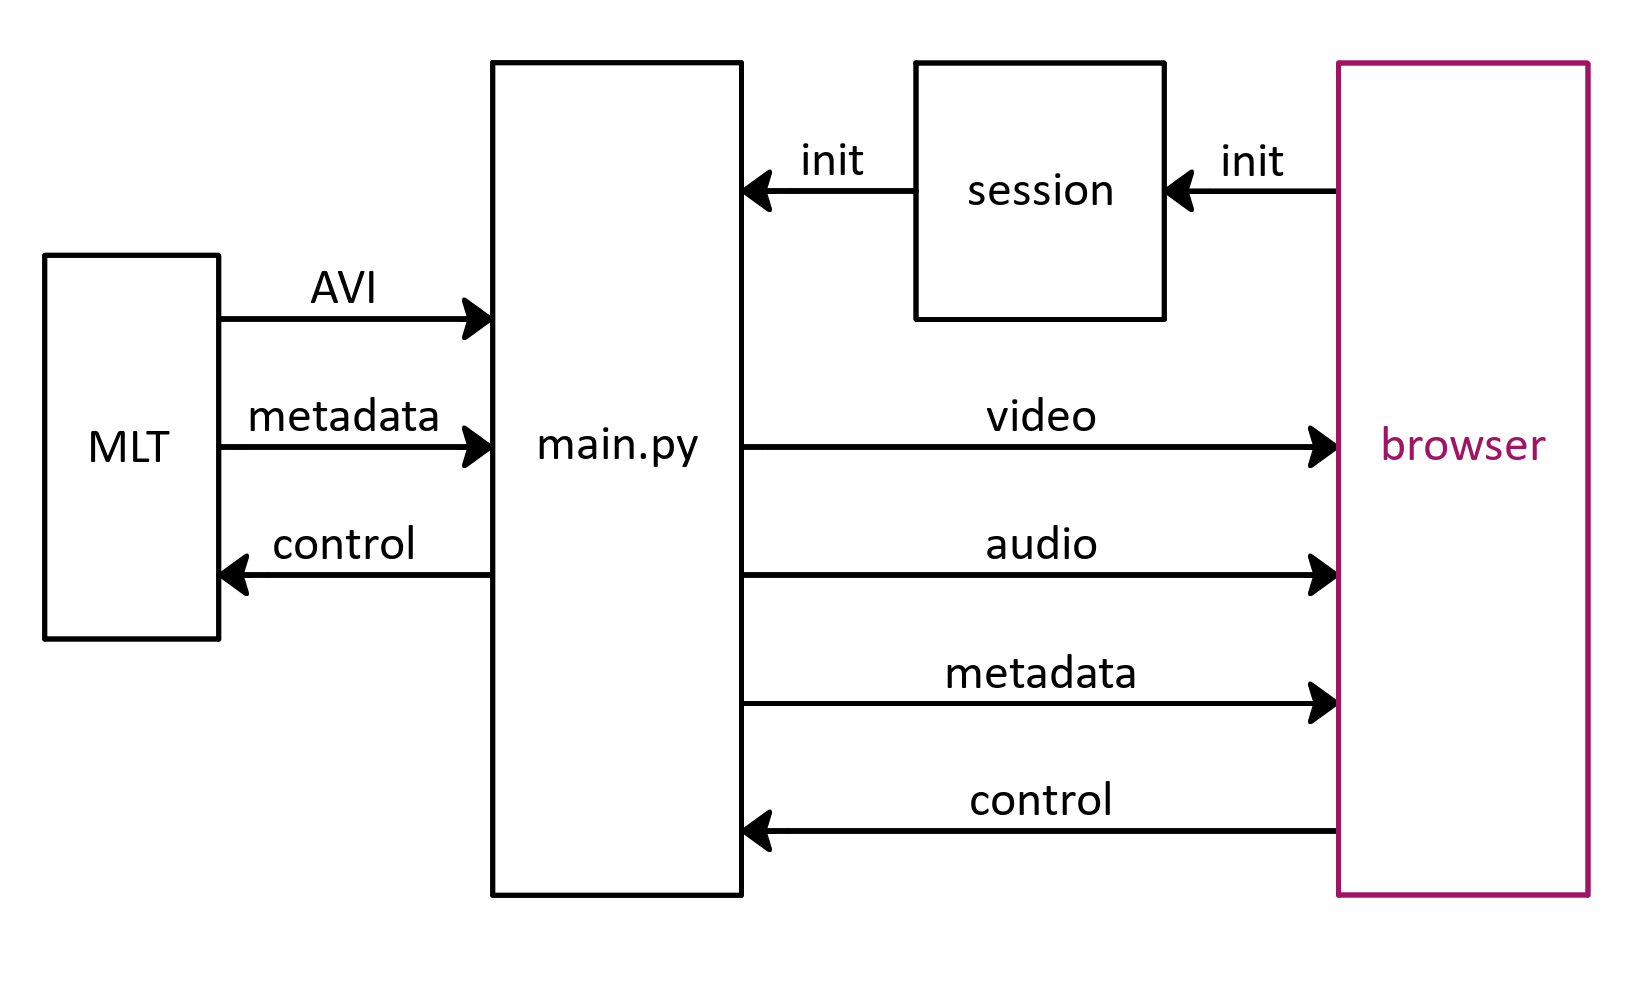
\includegraphics[width=0.5\textwidth]{IM_FE.png}
	\caption{Accurate Video in the system architecture}
\end{figure}













%-------------------------------------------------------------------------------------------------------
\subsection{JIT-WebRTC} \label{subsection:jit-webrtc}
% Describe the backend

The following description of the system is based on the code base and the information from the \texttt{README} file~\cite{RM_Backend}.

JIT-WebRTC is a live transcoder with a WebRTC output. As described in Section~\ref{subsection:technicalbackground}, transcoding is the conversion of one digital data format into another.~\cite{transcoding}

%# jit-webrtc
%
%Live Transcoder with WebRTC output
%

The backend consists of three components that will be described in the following:
\begin{itemize}
	\item Melt
	\item \texttt{main.py}
	\item Session service
\end{itemize}

The system's frontend was described in Section \ref{subsection:accuratevideo}

\begin{figure}[H]
	\centering
	
\includegraphics[width=0.8\textwidth]{IM3.png}
	\caption[System architecture]{Architecture of the system that consits out of four parts.}
\end{figure}

%## Design 
%
%The system consists of four "moving parts": three on the backend (`melt`, `main.py` and `session-service`)
%and one on the frontend (website with a JavaScript/WebRTC client).
%
%```
%                  +---------+      +---------+      +---------+
%                  |         | init |         | init |         |
%                  |         |<-----| session |<-----|         |
%+------+   AVI    |         |      |         |      |         |
%|      |--------->|         |      +---------+      |         |
%|      | metadata |         |         video         |         |
%| melt |--------->| main.py |---------------------->| browser |
%|      | control  |         |         audio         |         |
%|      |<---------|         |---------------------->|         |
%+------+          |         |        metadata       |         |
%                  |         |---------------------->|         |
%                  |         |        control        |         |
%                  |         |<----------------------|         |
%                  +---------+                       +---------+
%```
%



%---------------------------------
\subsubsection{Melt}

\begin{CountingDefinition}[Melt framework]{def:melt}
	
	The Melt framework (MLT/Melt) is a multimedia framework that is commonly used for video editing and playback. It provides a set of tools, libraries, and services for handling multimedia content, including video and audio.~\cite{melt} 
		
\end{CountingDefinition}

TODO

\begin{itemize}
	\item \texttt{melt.c} file
	\item Melt is used to decode input files and perform rendering
	\item It is the command line interface (CLI) for the MLT framework.
\end{itemize}





%---------------------------------
\subsubsection{Data flow}

The user initiates a session through the browser, which then initiates the \texttt{main.py} script.
Control commands are then sent from the browser to \texttt{main.py} with a WebRTC data channel.

From the \texttt{main.py}, the control commands get sent to Melt via \texttt{stdout} (standard output) and \texttt{stdin} (standard input). These are the default input and output channels, that allow the Python script communication with other components.
Data written to \texttt{stdout} by the Python code can be captured or redirected and data from an external source can be read from \texttt{stdin} by the Python script. \cite{python}

\begin{figure}[H]
	\centering
	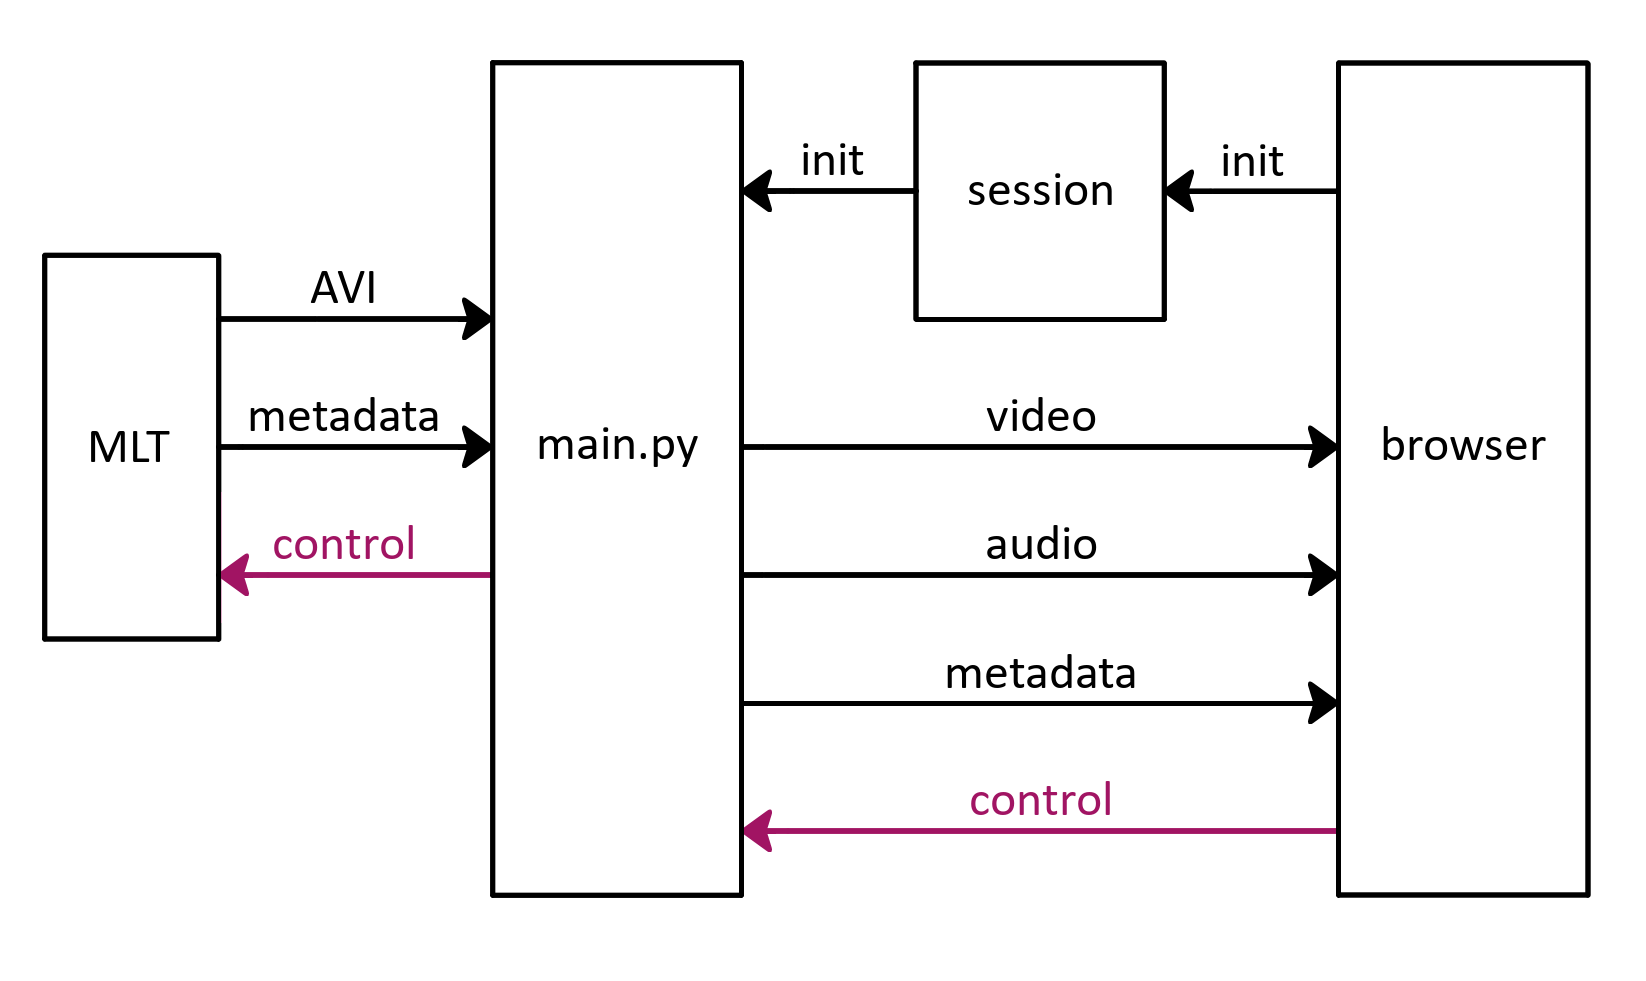
\includegraphics[width=0.5\textwidth]{IM_control.png}
	\caption{Control commands in the system architecture}
	
\end{figure}


Melt sends an AVI stream with the rendered video and audio to the \texttt{main.py} via a named pipe and status messages and metadata via another named pipe.
AVI is a file format that can contain audio and video information to allow synchronized playback of audio and video components.~\cite{avi} AVI was further described in Section~\ref{subsection:technicalbackground} and named pipes in Section~\ref{subsection:technicalbackground}.

\begin{figure}[H]
	\centering
	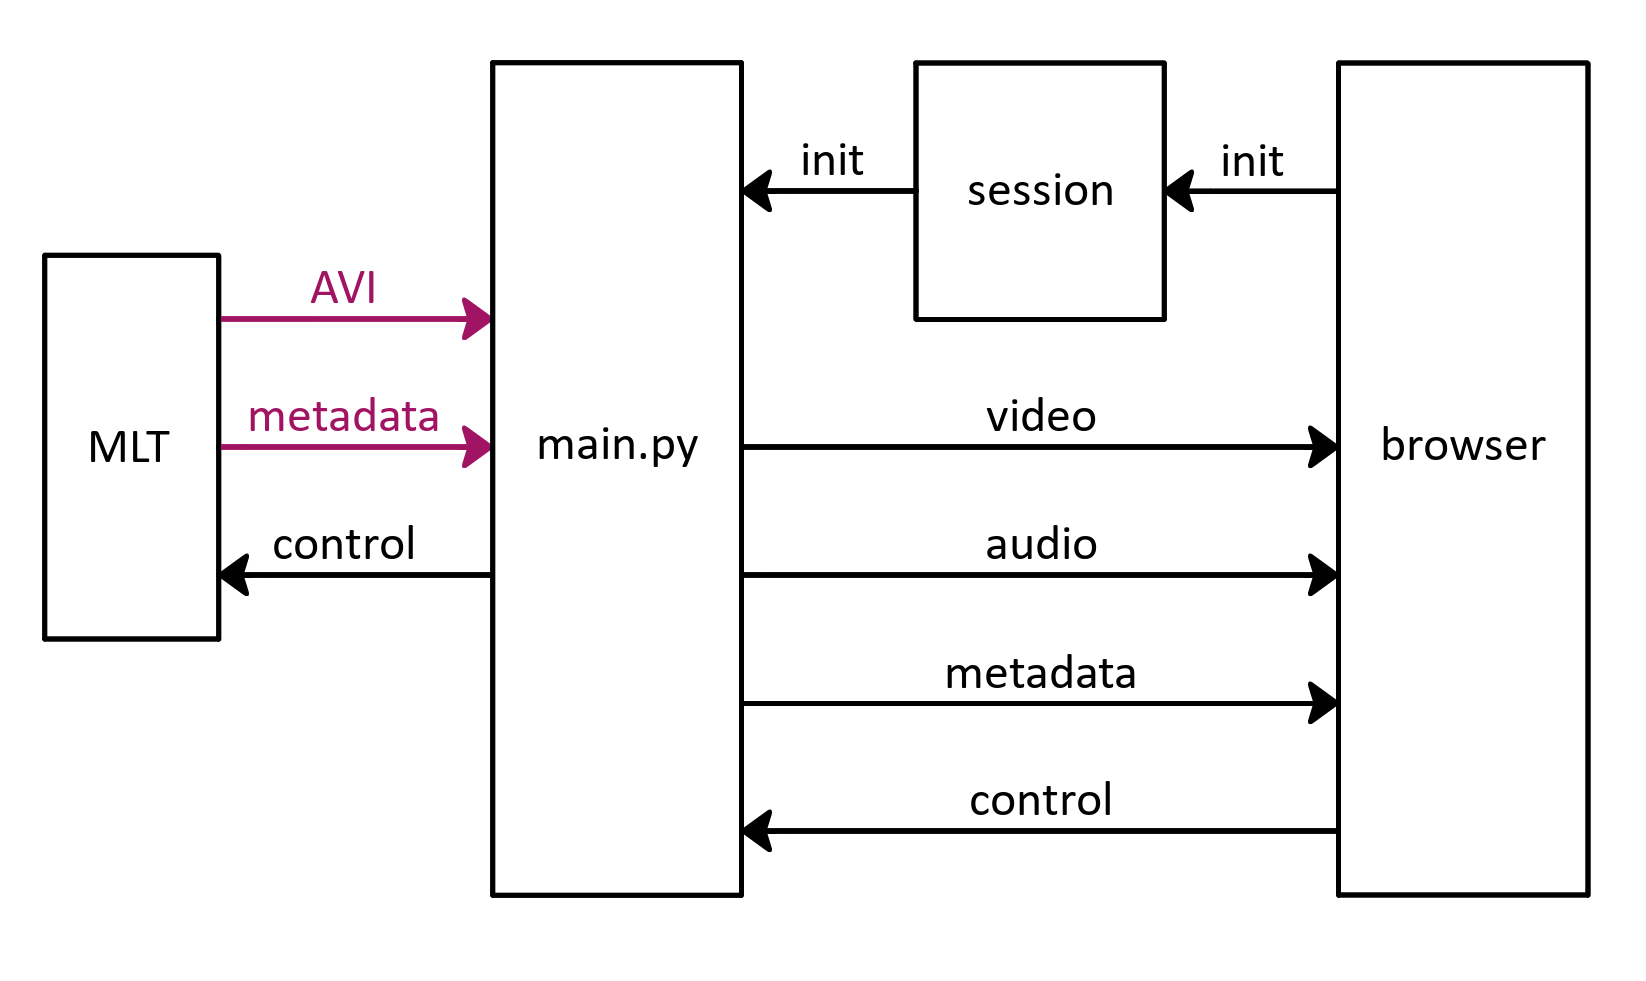
\includegraphics[width=0.5\textwidth]{IM_avi.png}
	\caption{AVI stream in the system architecture}
\end{figure}


Then the audio and video from the incoming AVI stream is extracted by the \texttt{main.py} script to then encode it for sending it to the browser with WebRTC. The WebRTC connection serves as a direct communication channel between the browser and the backend, enabling real-time data exchange, involving audio, video, or other data streams. 

TODO: Is is encoded into h-264 here?

%It has the ability to extract specific channels from the rendered audio, to %be rendered to an stereo stream for WebRTC.
%It does not appear to be possible to encode surround sound for WebRTC, despite WebRTC using the Opus codec which is surround capable.
%This may be a limitation in `aiortc`, in WebRTC or in the browser, or all three.
%

\begin{figure}[H]
	\centering
	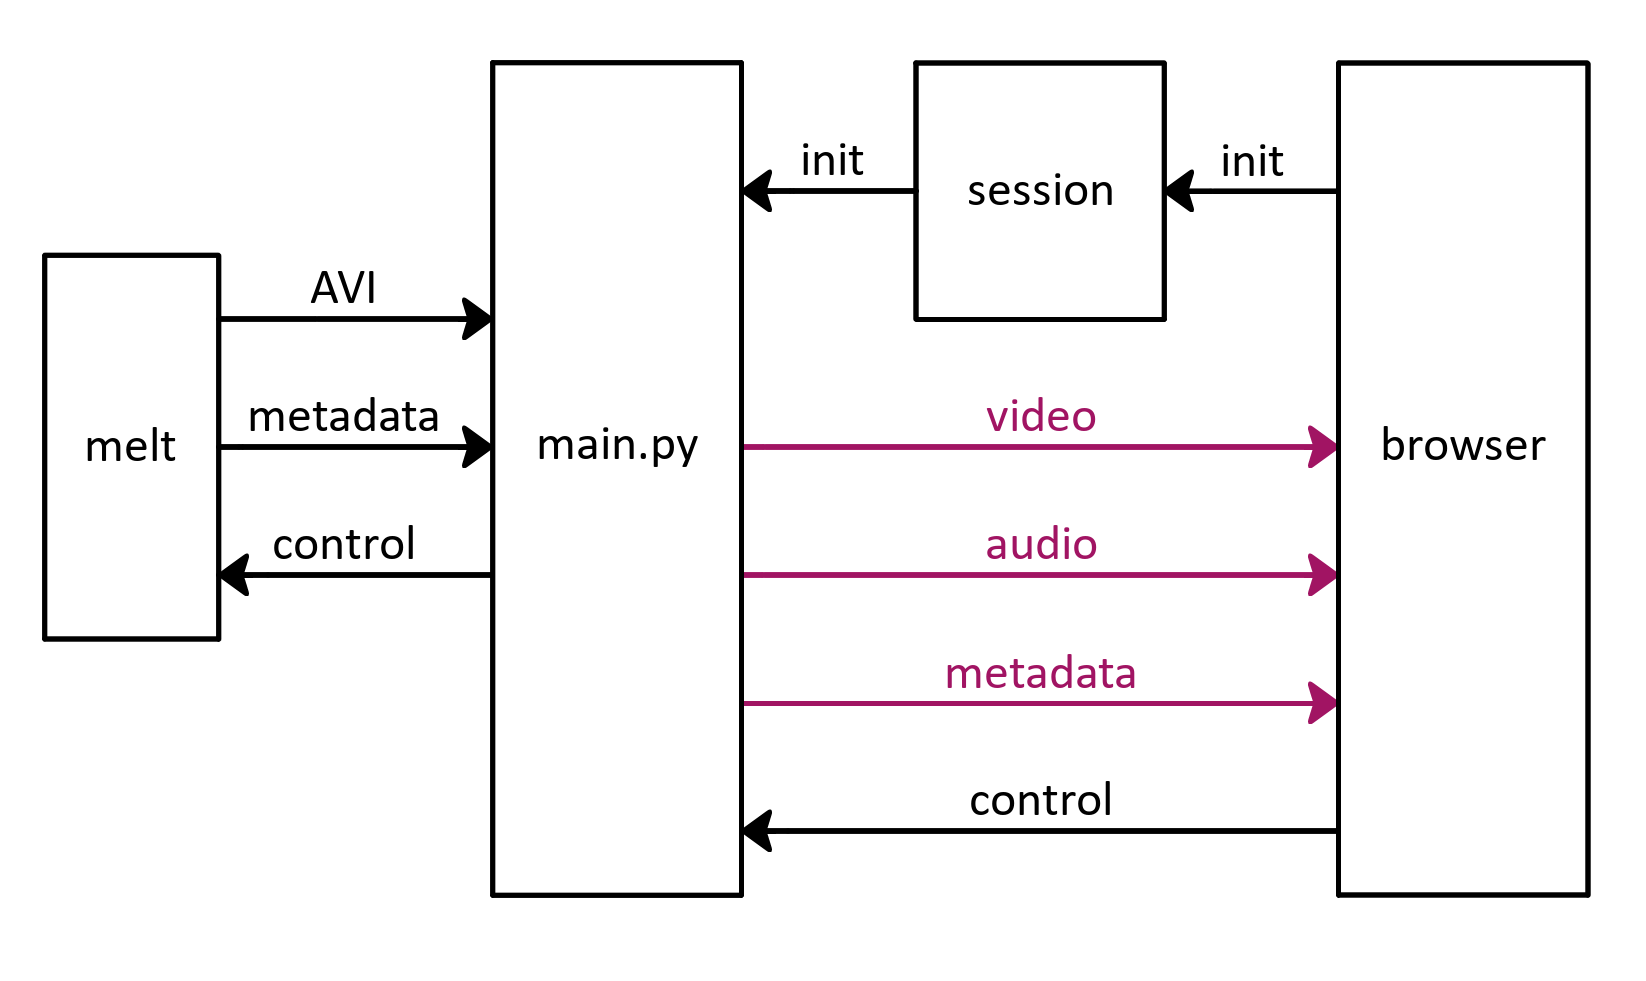
\includegraphics[width=0.5\textwidth]{IM_wrtc.png}
	\caption{WebRTC connection in the system architecture}
\end{figure}

Then the JavaScript client of the browser receives the video and audio and plays it. In addition to this, it
receives metadata from the \texttt{main.py} script and sends commands and ping responses over the control channel.


\begin{figure}[H]
	\centering
	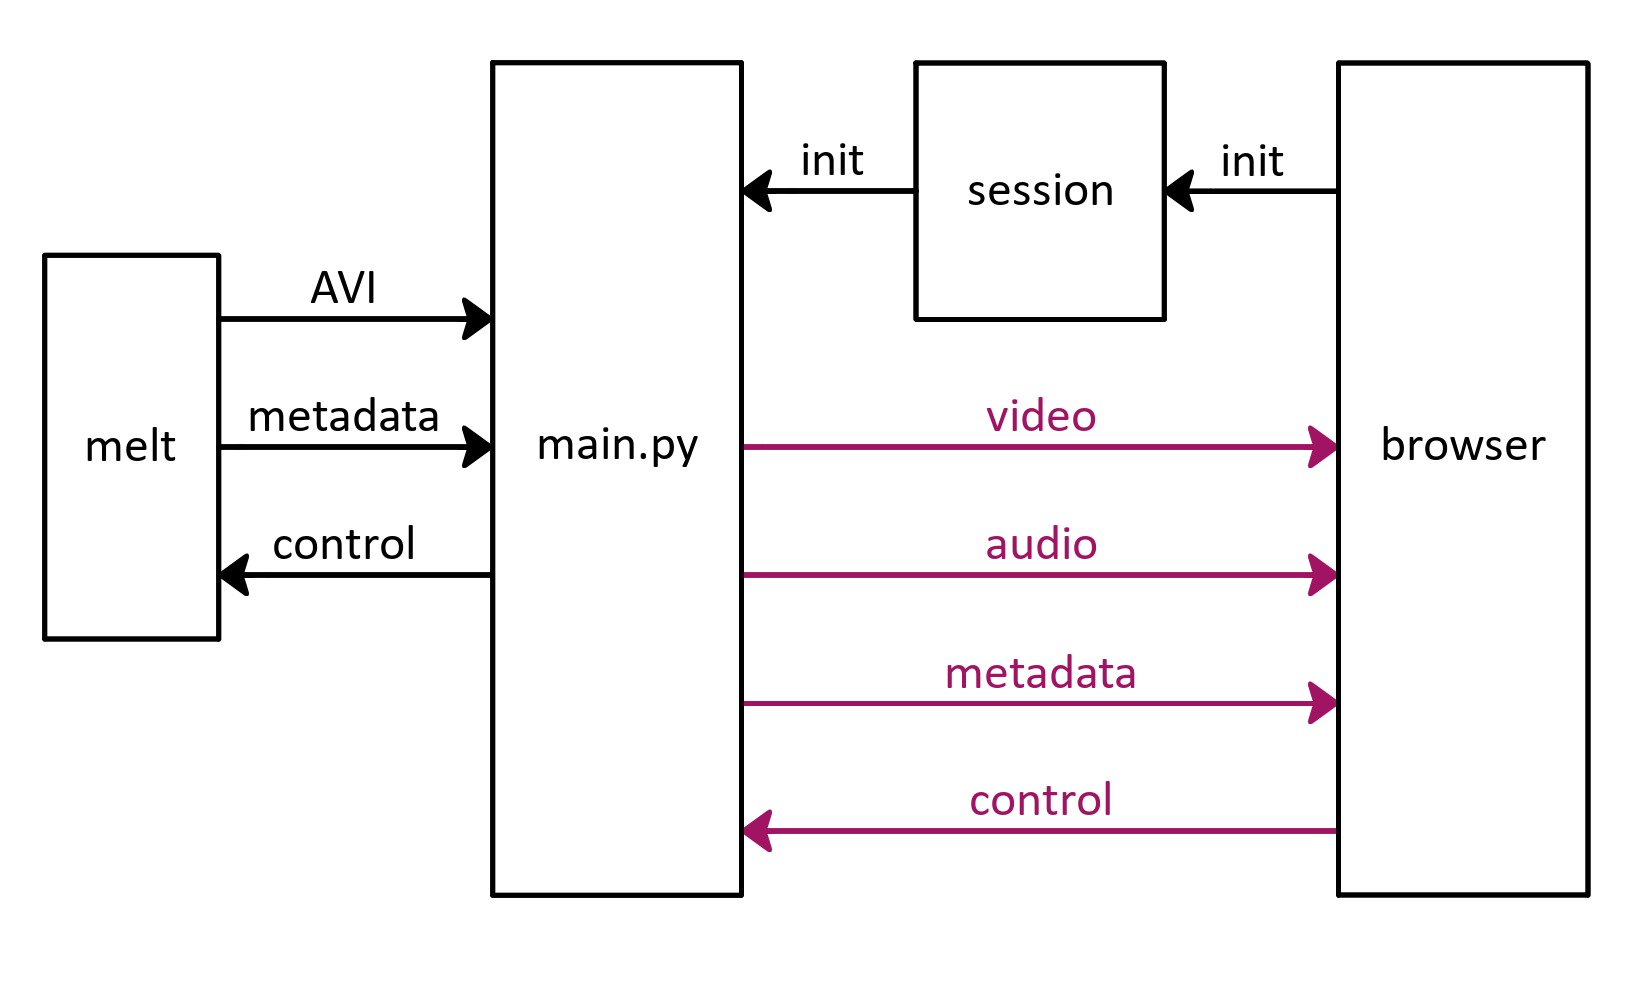
\includegraphics[width=0.5\textwidth]{IM_wrtc_control.png}
	\caption[WebRTC and control in the system architecture]{WebRTC connection and control commands in the system architecture}
\end{figure}

Melt and the \texttt{main.py} script are started once for each JIT session with a parameter that presents the media from the start on.

%`main.py` and `melt` is started once for each JIT session, and media is presented to it on startup. 

\subsubsection{Session}

\texttt{Session} is a java-based service, designed to support machine-to-machine interaction between the browser and the backend (\texttt{main.py} and Melt). Web services allow different applications, that often run on different platforms and are written in different programming languages, to communicate with each other.~\cite{webservice}

The \texttt{Session} service exposes a REST API (described in Section~\ref{subsection:technicalbackground}) for initiating a JIT session with specified media details. 

% Additionally, it leverages AWS, specifically utilizing the Auto Scaling Group (ASG) feature to manage a cluster of instances dynamically, ensuring scalability and efficient distribution of JIT sessions across the instances in the cluster.

% AWS
%2. **AWS (Amazon Web Services):**
%- **Definition:** AWS is a cloud computing platform provided by Amazon. It offers a wide range of services, including computing power, storage, databases, machine learning, and more, allowing businesses to scale and grow without the need for significant upfront investments in physical infrastructure.

% ASG cluster
%3. **ASG Cluster (Auto Scaling Group):**
%- **Definition:** An Auto Scaling Group is an AWS service that automatically adjusts the number of compute instances (e.g., virtual machines) in response to changes in demand or other specified conditions. It helps ensure that the desired number of instances are available to handle varying workloads.



%`session` is a Java-based service that presents a REST api that can be used to start a new JIT session given a description of the media to use. It also has support for managing a full ASG cluster on AWS, and distribute new JIT sessions on the instances in 
%the ASG.
%
%For more information on each component see:
%* [`melt`](https://github.com/sirf/mlt.git)
%* [`main.py`](jit/README.md)
%* [`session`](session/README.md)
%

For development and quick testing without the session service, JIT can be started in a Docker container. A Docker container is in isolated environment in which an application can be run and Docker is the platform that enables the usage of those containers.~\cite{docker}


\begin{figure}[H]
	\centering
	
\includegraphics[width=0.6\textwidth]{IM2.png}
	\caption{System architecture when run in a docker container.}
\end{figure}


%## Development
%
%For development and quick testing without the session service, on can either start JIT as a docker, or run JIT directly on your computer. The latter has some problems if you're on an Apple ARM.
%
%Run the docker:
%
%`docker/main/main.sh --threads 16 --port 8080 $VIDEOFILE`
%
%Where `$VIDEOFILE` is either a local path or a URL. `threads` and `port` are both optional, with current default values set to 72 threads and port 8080.
%
%To run JIT directly, see [`jit/README.md`](jit/README.md).
%
%### Open Docker IPs
%
%Your Docker container will get an IP in the style of 172.17.0.\*. Using e.g. Docker CE on Linux this IP will be reachable from outside the container. However, on Docker Desktop for Mac, this IP will not be opened. This will cause problems. There is a service that can fix this. You **install and activate it once** by doing this:
%
%```
%# Install via Homebrew
%brew install chipmk/tap/docker-mac-net-connect
%
%# Run the service and register it to launch at boot
%sudo brew services start chipmk/tap/docker-mac-net-connect
%```
%
%
%## Deployment
%
%Currently the only way supported for deployment is by using EC2 instances on AWS. An AMI is created by CI on release, containing a 
%local instance of the `session-service`, together with `main.py`, `melt` and anything else needed to start JIT processes on the EC2 
%instance. For more information about what the AMI contains, and how configuration can be fed to it see [`ami/README.md`](ami/README.md).
%
%### Terraform
%
%Terraform modules are supplied that simplify setup of either single EC2 instances or a full ASG cluster of instances, including 
%`session-service` running as an orchestrator on ECS. See [`terraform/README.md`](terraform/README.md) for more information on 
%available modules, their parameters and outputs.
%






%-------------------------------------------------------------------------------------------------------
\subsection{Technology} \label{subsection:technology}
% Discuss the technologies and tools chosen for the implementation.







%-------------------------------------------------------------------------------------------------------
\subsection{Melt Filter} \label{subsection:meltfilter}


Use of \texttt{avfilter.colorchannelmixer}:

\url{https://www.mltframework.org/plugins/FilterAvfilter-colorchannelmixer/}

\texttt{title: colorchannelmixer \newline
	media types: Video \newline
	description: Adjust colors by mixing color channels.}

Execution of \texttt{melt https://s3.eu-central-1.amazonaws.com/accurate-player\--demo-assets/timecode/sintel-2048-timecode-stereo.mp4 \\ -filter avfilter.colorbalance av.rs=1 av.gm=1 av.bh=1}:


\begin{minipage}{0.5\textwidth}
	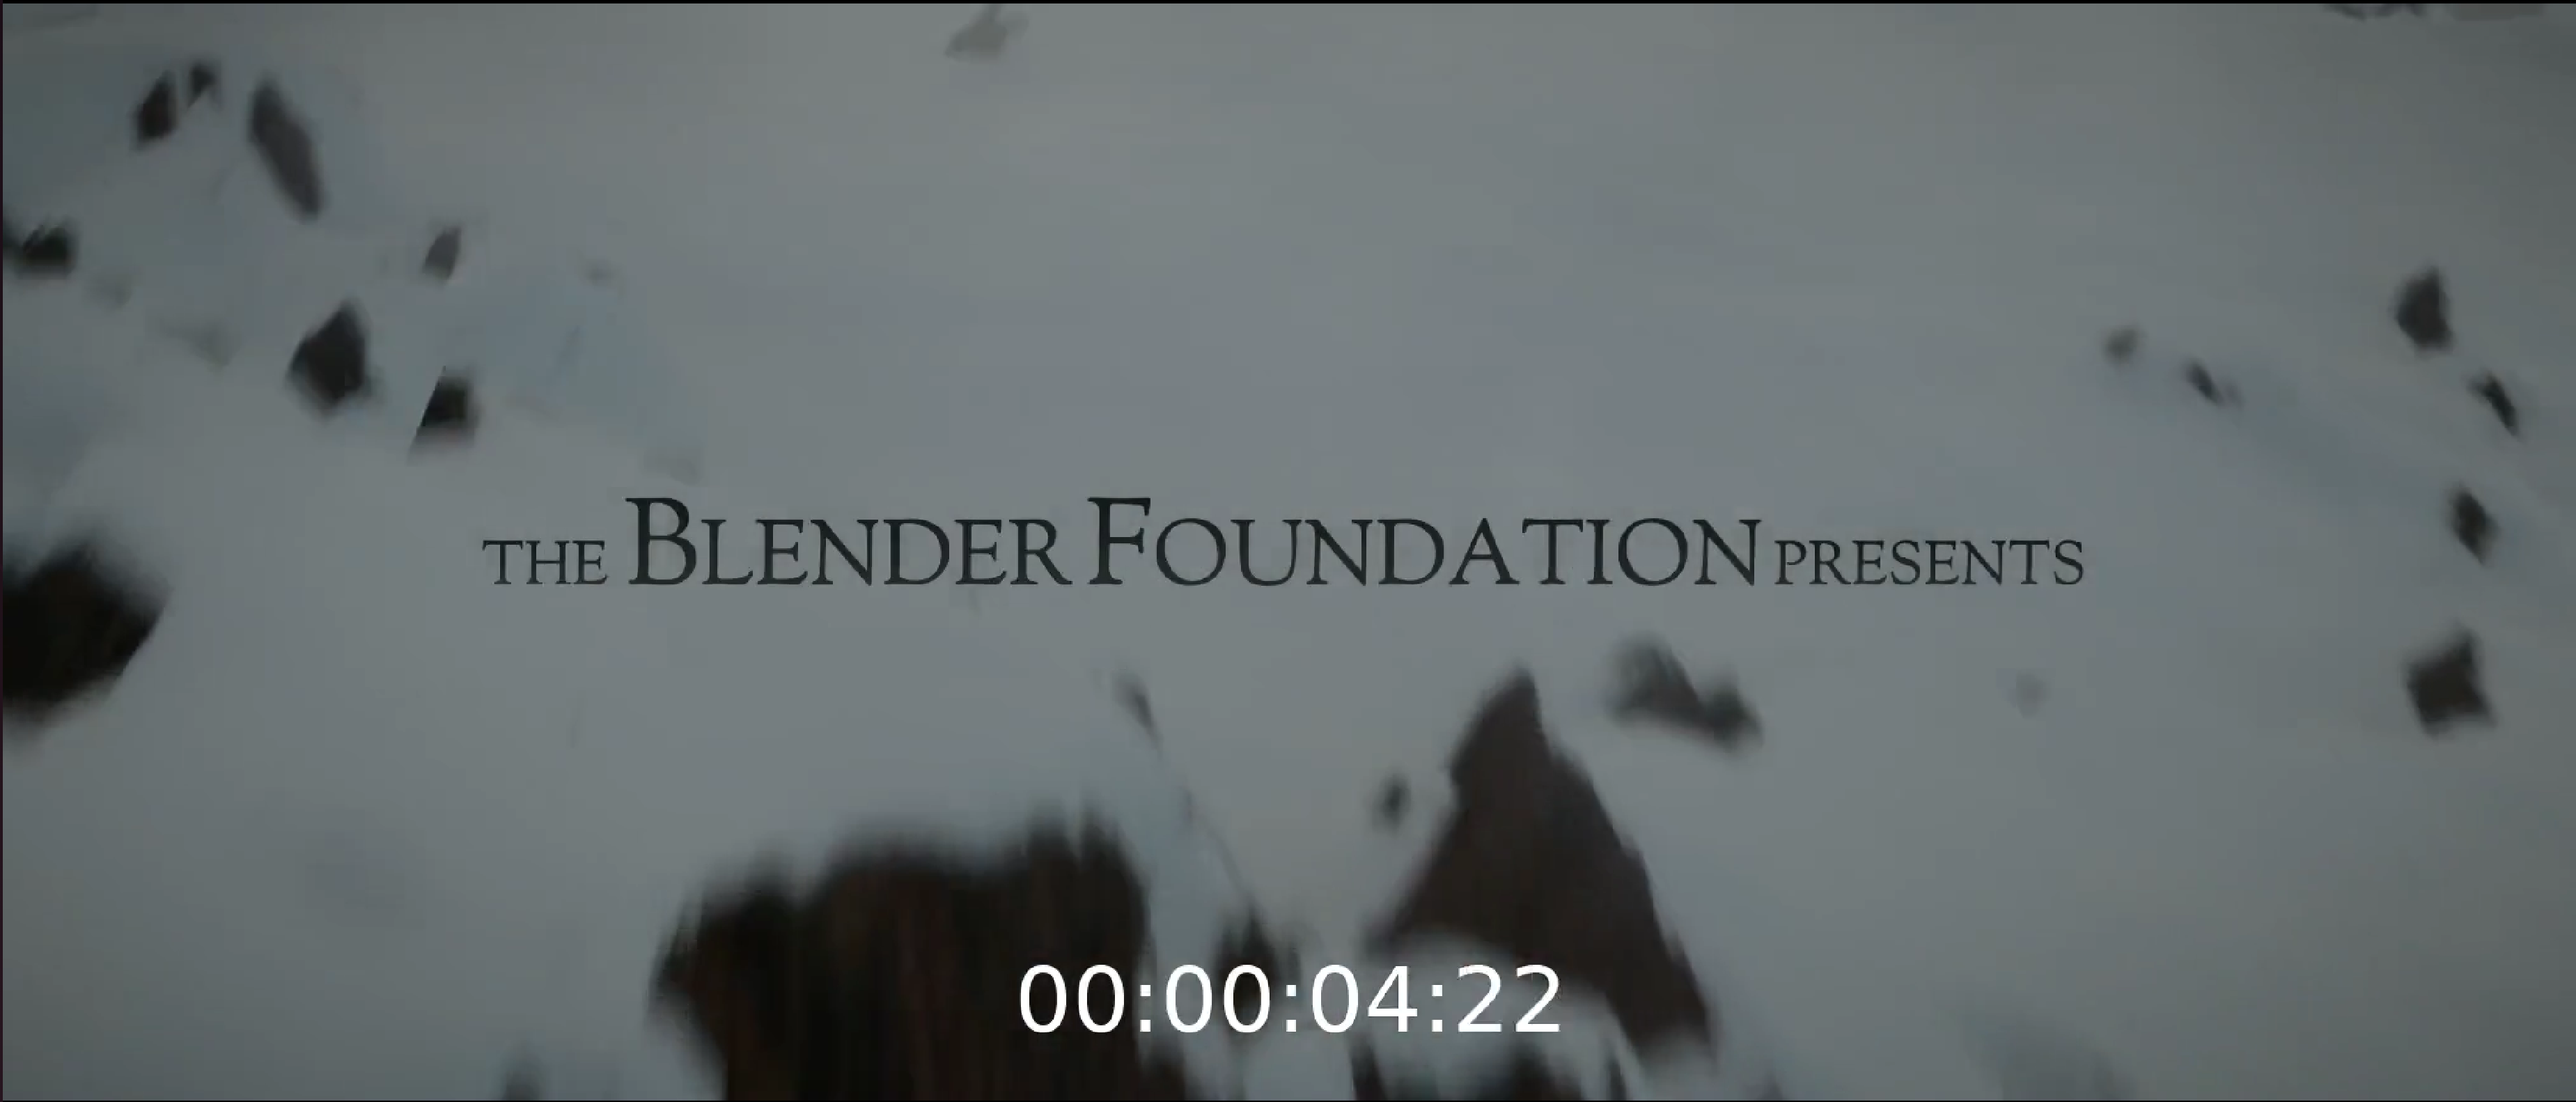
\includegraphics[width=0.9\textwidth]{colourdefault.png}
	Original colours
\end{minipage}\begin{minipage}{0.5\textwidth}
	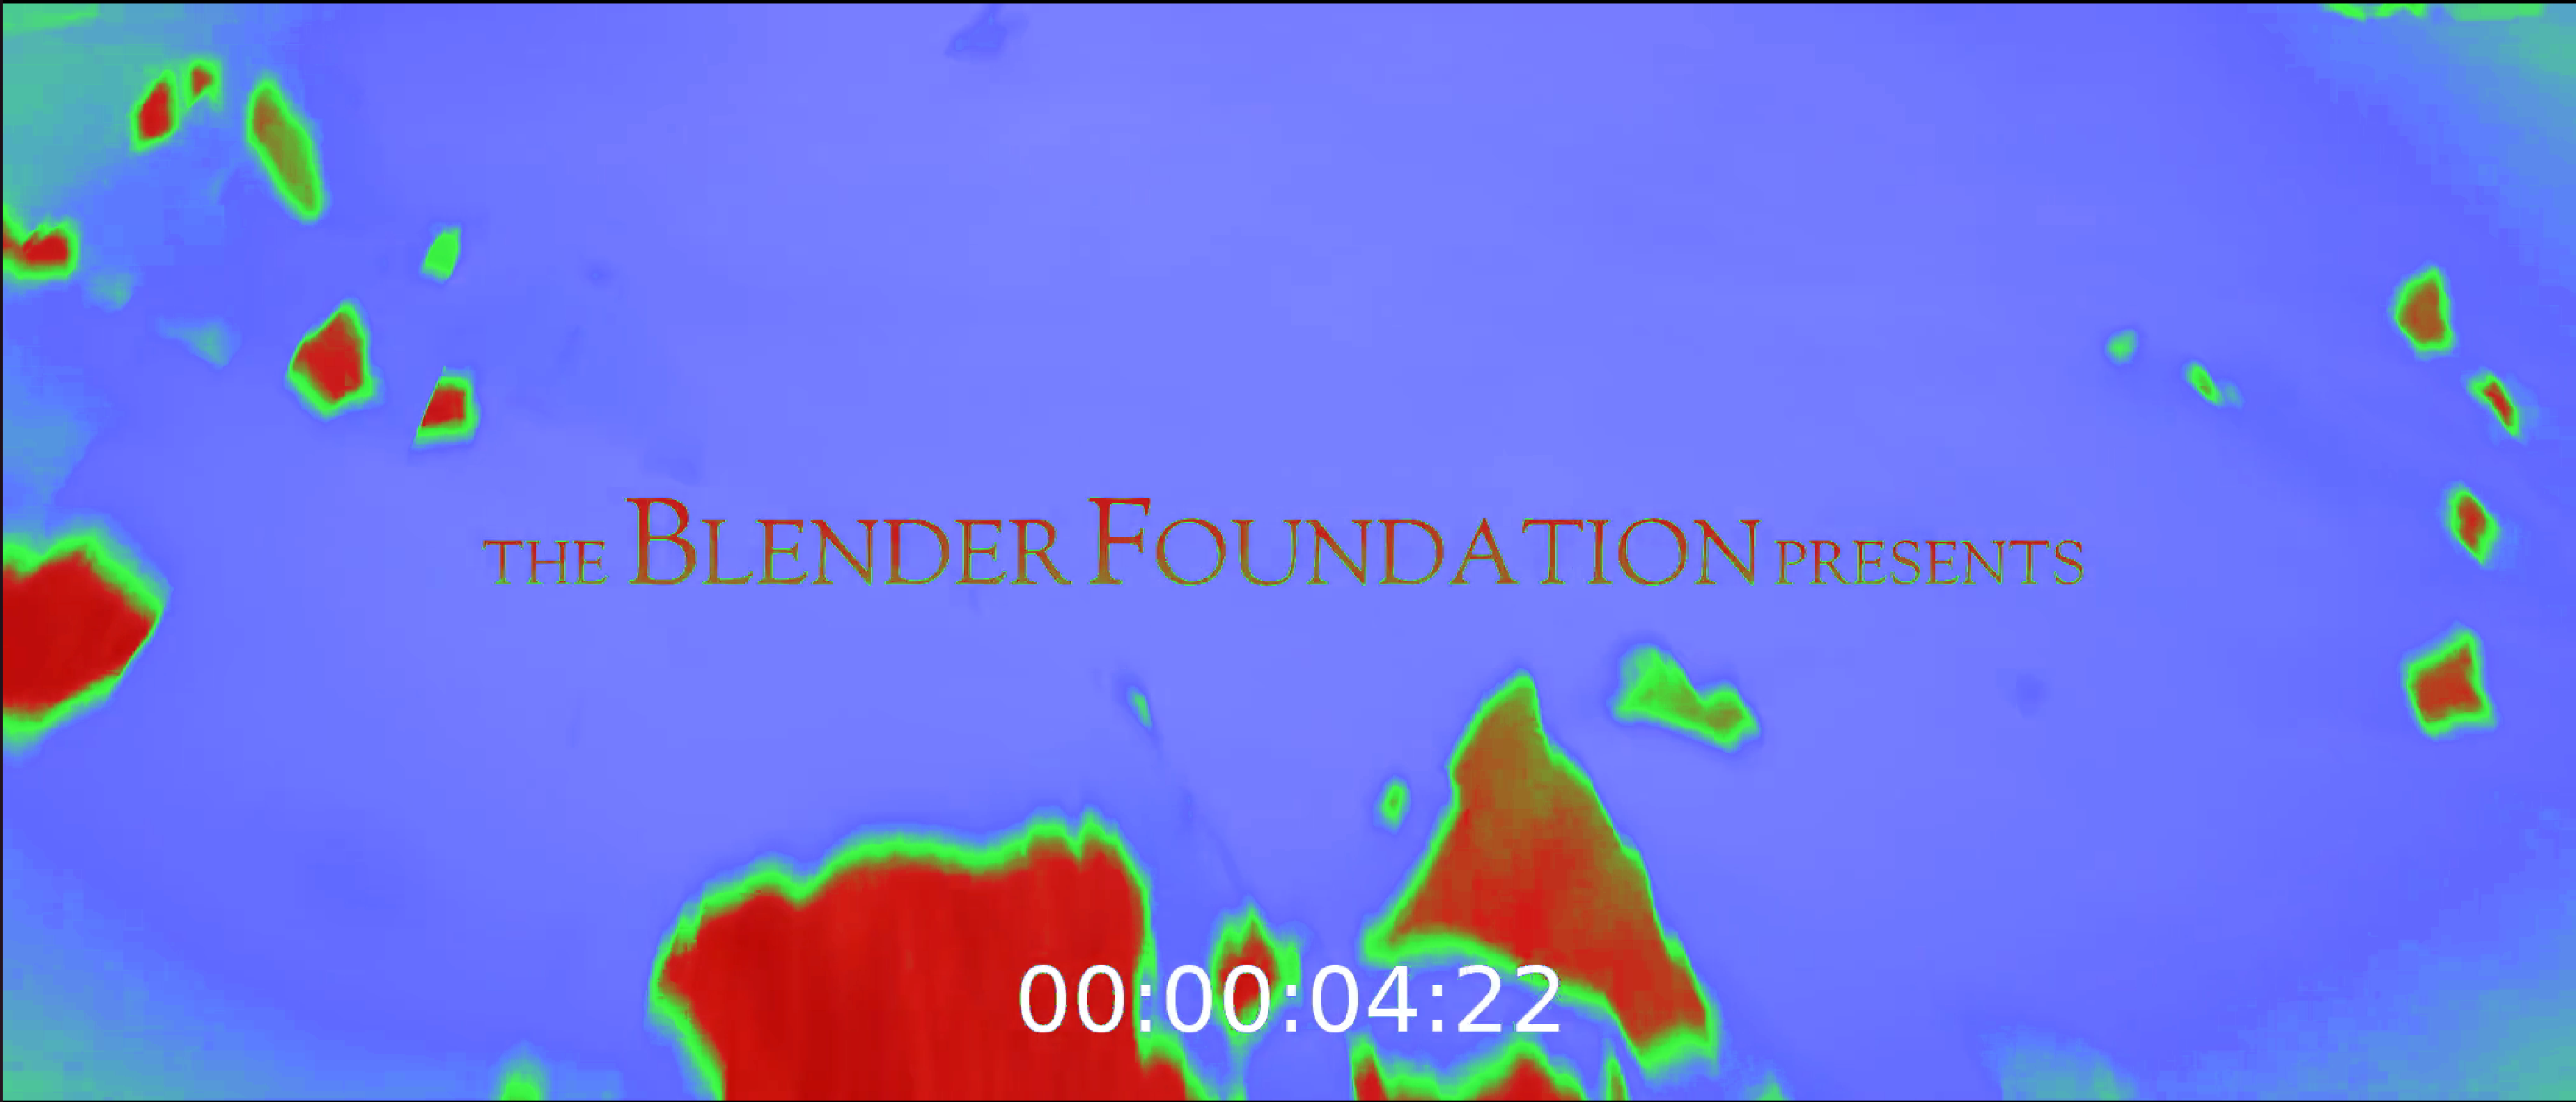
\includegraphics[width=0.9\textwidth]{colourhigh.png}
	Colours with \texttt{av.rs=1} \texttt{av.gm=1} \texttt{av.bh=1}
\end{minipage}

Adding filter to \texttt{local\_melt.py} to execute it in the Accurate Player using JIT:
`
\begin{center}
	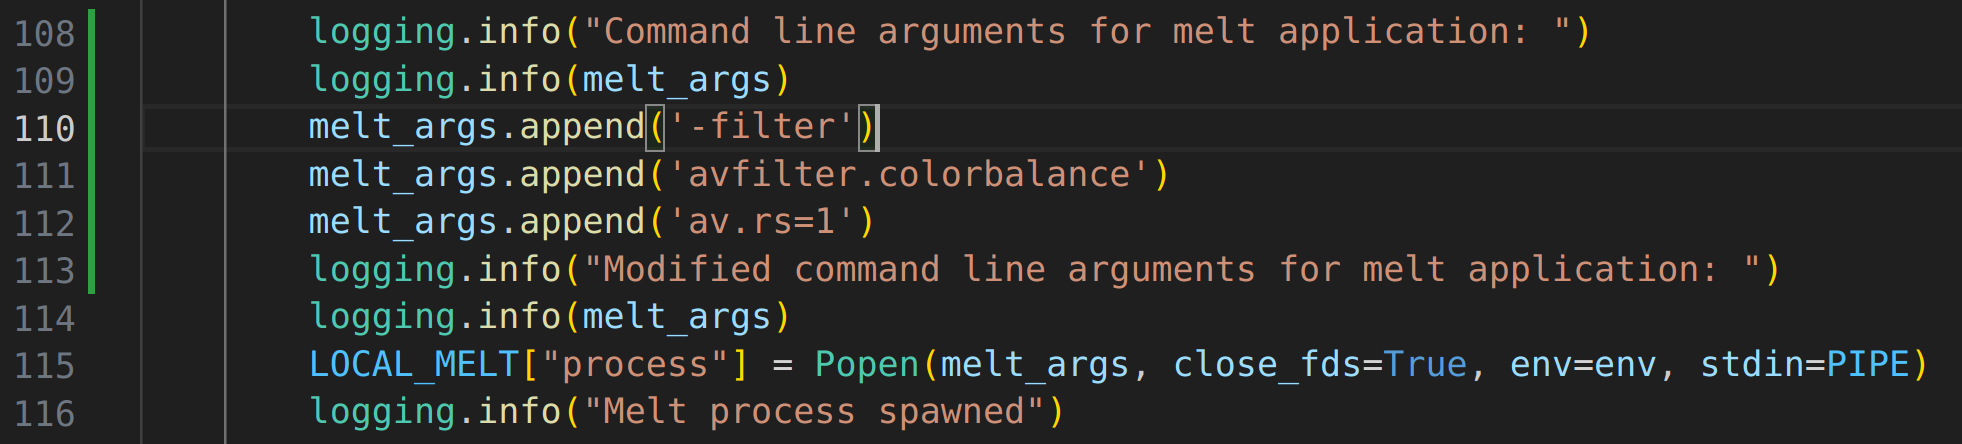
\includegraphics[height=0.13\textwidth]{code.png}
	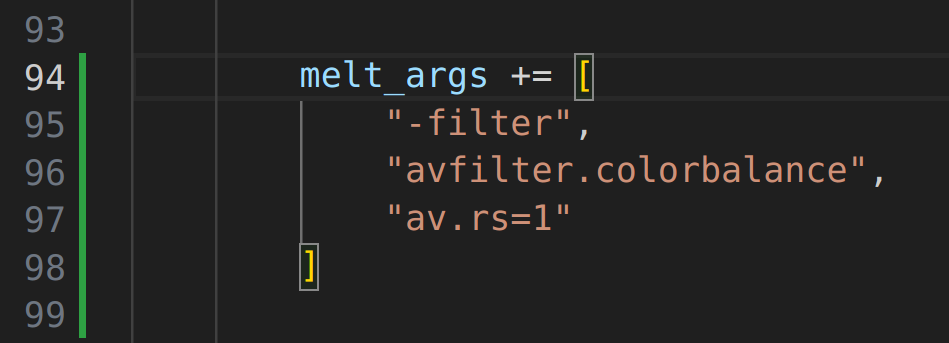
\includegraphics[height=0.13\textwidth]{codecleaner.png}
\end{center}

\begin{center}
	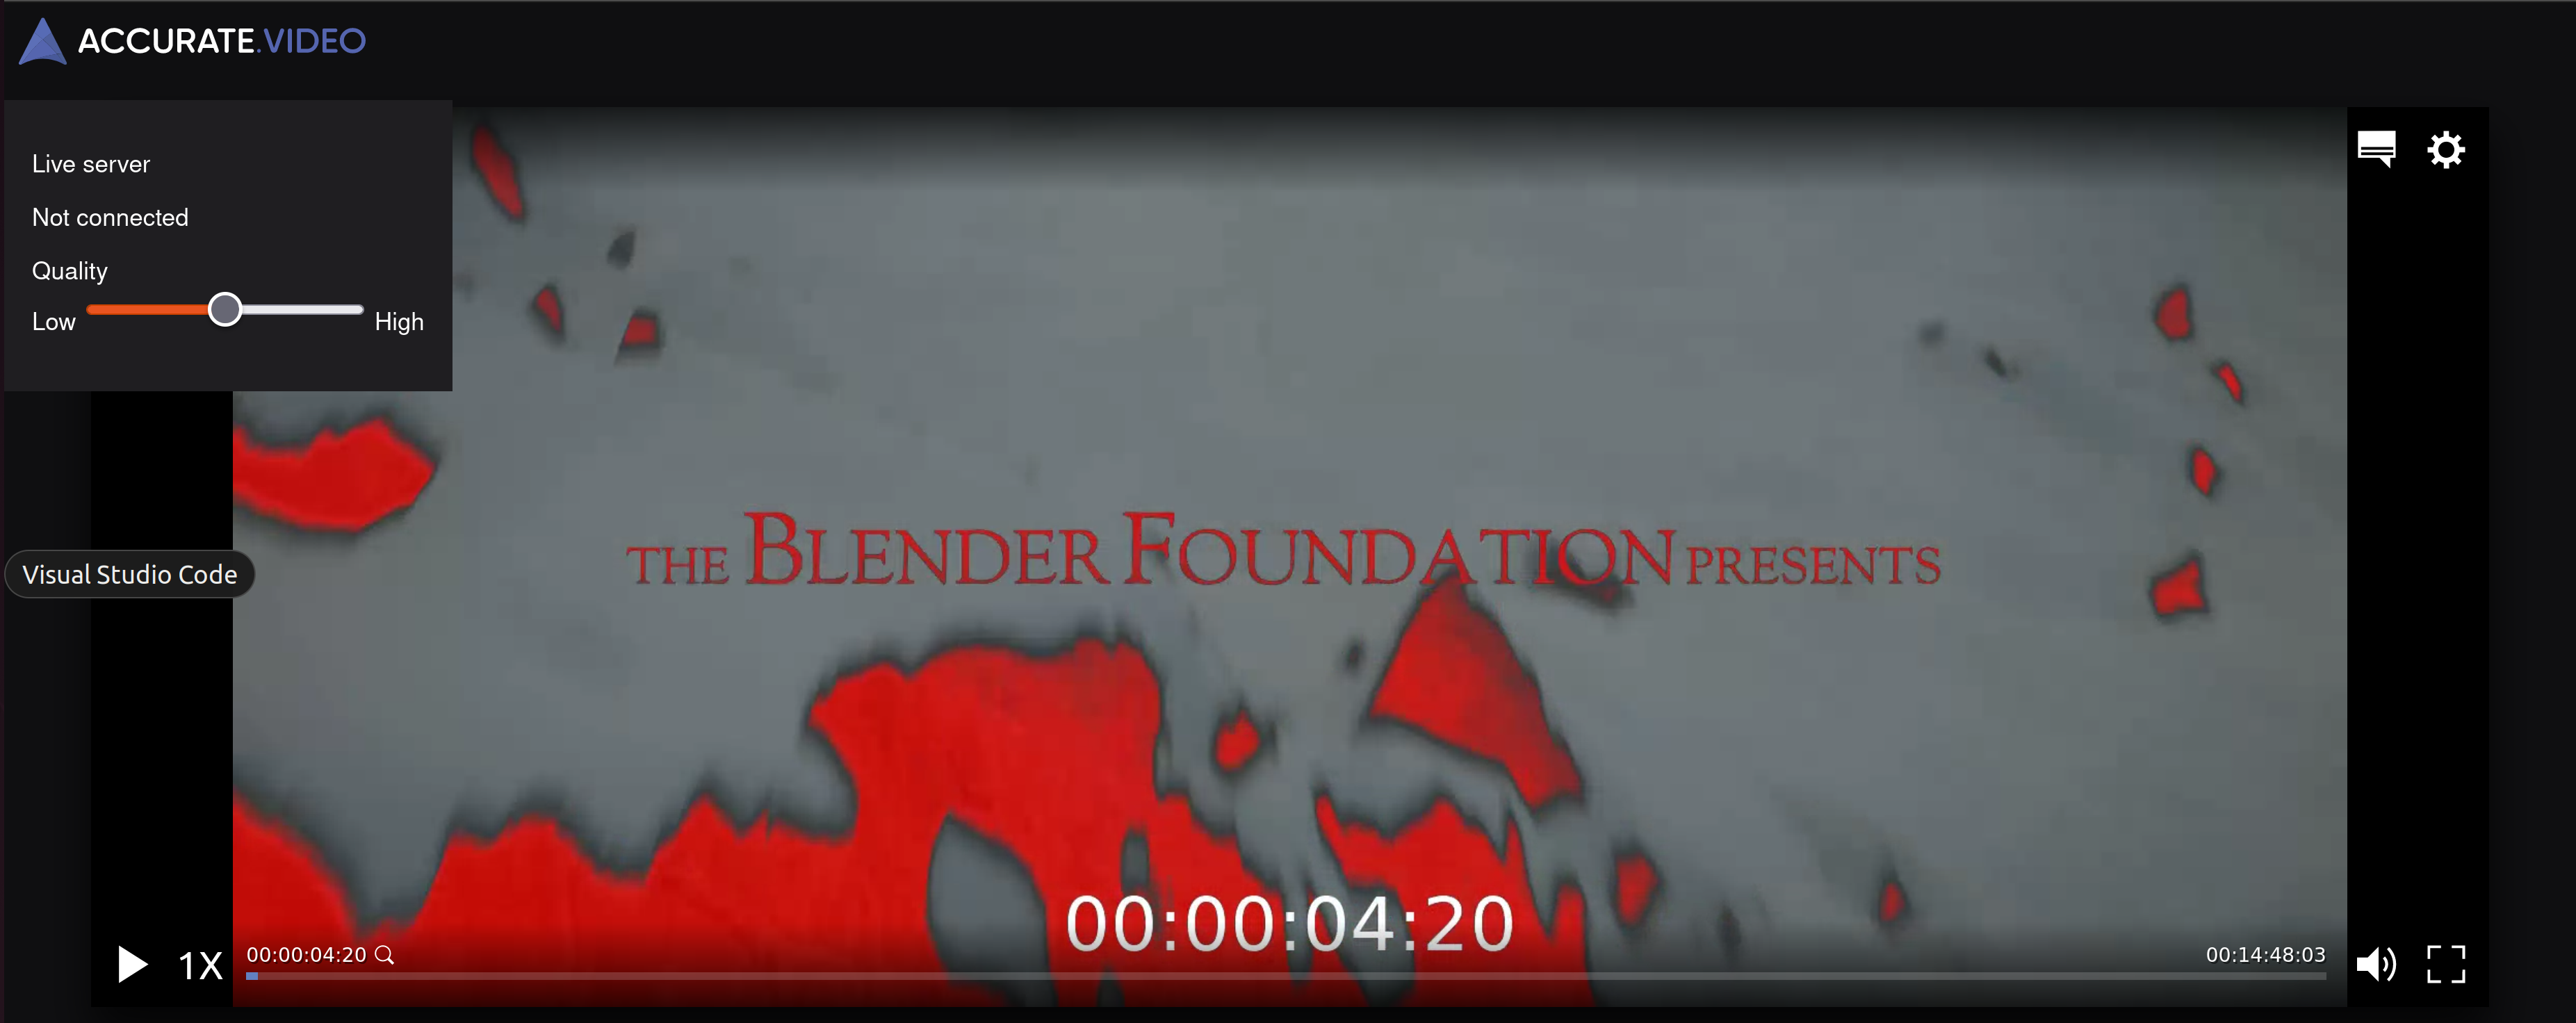
\includegraphics[width=0.8\textwidth]{ap_red.png}
\end{center}




%
%
%
%
%=======================================================================================================
%
%
%
%
%=======================================================================================================
% CHAPTER: RESULTS AND EVALUATION
%=======================================================================================================
\newpage
\section{Experimental Evaluation and Discussion} \label{section:experimentalevaluationanddiscussion}


%-------------------------------------------------------------------------------------------------------
\subsection{Testing} \label{subsection:testing}
% Discuss the testing methodologies and present validation results.


%-------------------------------------------------------------------------------------------------------
\subsection{Evaluation and Comparison} \label{subsection:evaluationandcomparison}
% Evaluate the system's performance against defined criteria.





%
%
%
%
%=======================================================================================================
%
%
%
%
%=======================================================================================================
% CHAPTER: CONCLUSION AND FUTURE WORK
%=======================================================================================================
\newpage
\section{Conclusion} \label{section:conclusion}


%-------------------------------------------------------------------------------------------------------
\subsection{Summary} \label{subsection:summary}
% Summarize the key findings and outcomes of the research.


%-------------------------------------------------------------------------------------------------------
\subsection{Contributions and Limitations} \label{subsection:contributionsandlimitations}
% Highlight your contributions to the field.
% Discuss any limitations encountered during the research.


%-------------------------------------------------------------------------------------------------------
\subsection{Future Work} \label{subsection:futurework}
% Suggest possible extensions or improvements to your work.





%
%
%
%
%=======================================================================================================
%
%
%
%
%=======================================================================================================
% REFERENCES
%=======================================================================================================
%\chapter*{References}
% Include a list of all references cited in the thesis.
	
	%-------------------------------------------------------------------------------------------	
	
	
	
	\newpage
	\addcontentsline{toc}{section}{References}
	\begin{spacing}{1}
		\printbibliography[notcategory=skipbibliography]
	\end{spacing}
	
	
	
%---------------------------------------------------------------------	
	
	
\newpage
\listoffigures



\newpage
\listoftables	
	
	
%---------------------------------------------------------------------

\appendix

\newpage

\section{README} \label{appendix:readme}


\subsection{Accurate-Player-3} \label{appendix:readmeaccurateplayer}

The README-file of the Accurate-Player-3 code was referenced as \cite{RM_Frontend} and is included for transparency in the following.

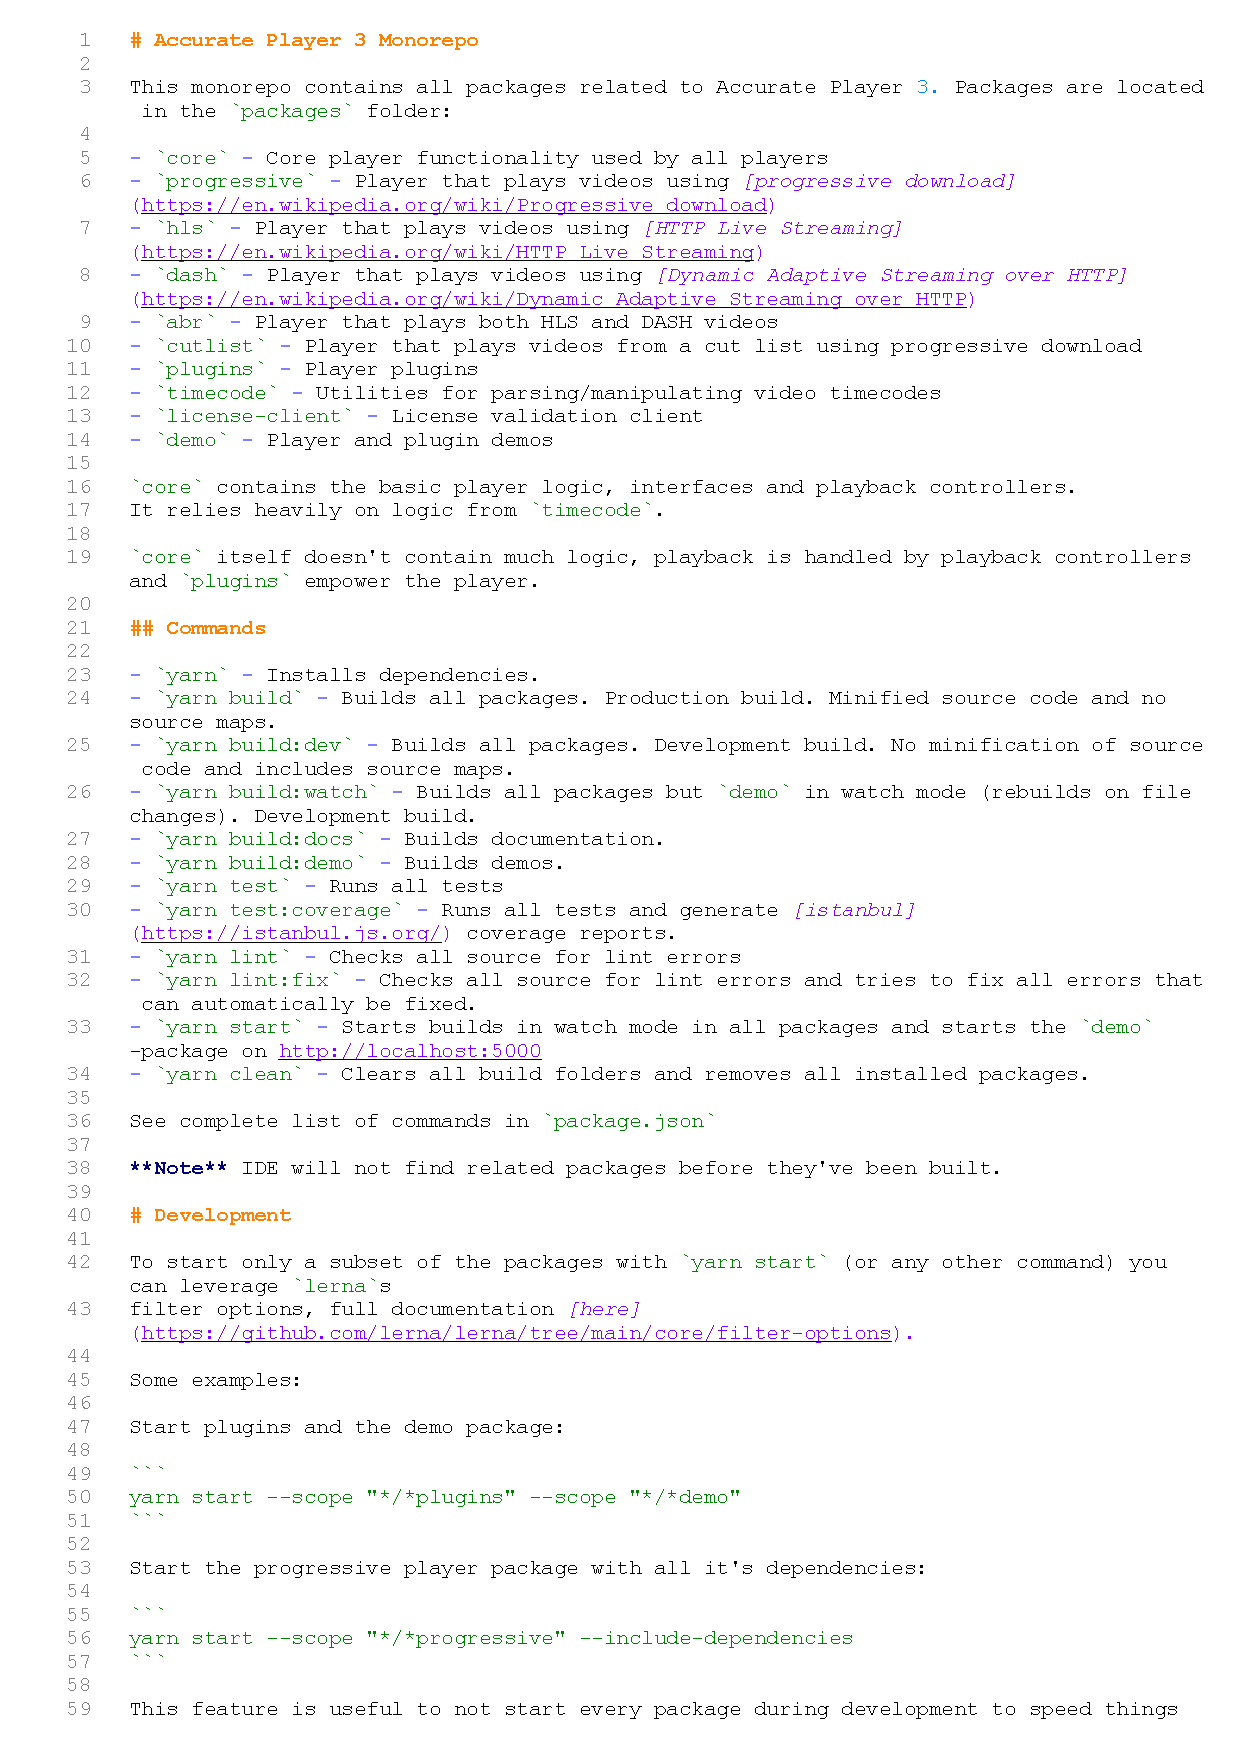
\includegraphics[page=1, width=0.9\textwidth]{FE.pdf}

\includegraphics[page=2, width=0.9\textwidth]{FE.pdf}



\newpage
\subsection{JIT-WebRTC} \label{appendix:readmejitwebrtc}

The README-file of the JIT-WebRTC code was referenced as \cite{RM_Backend} and is included for transparency in the following.

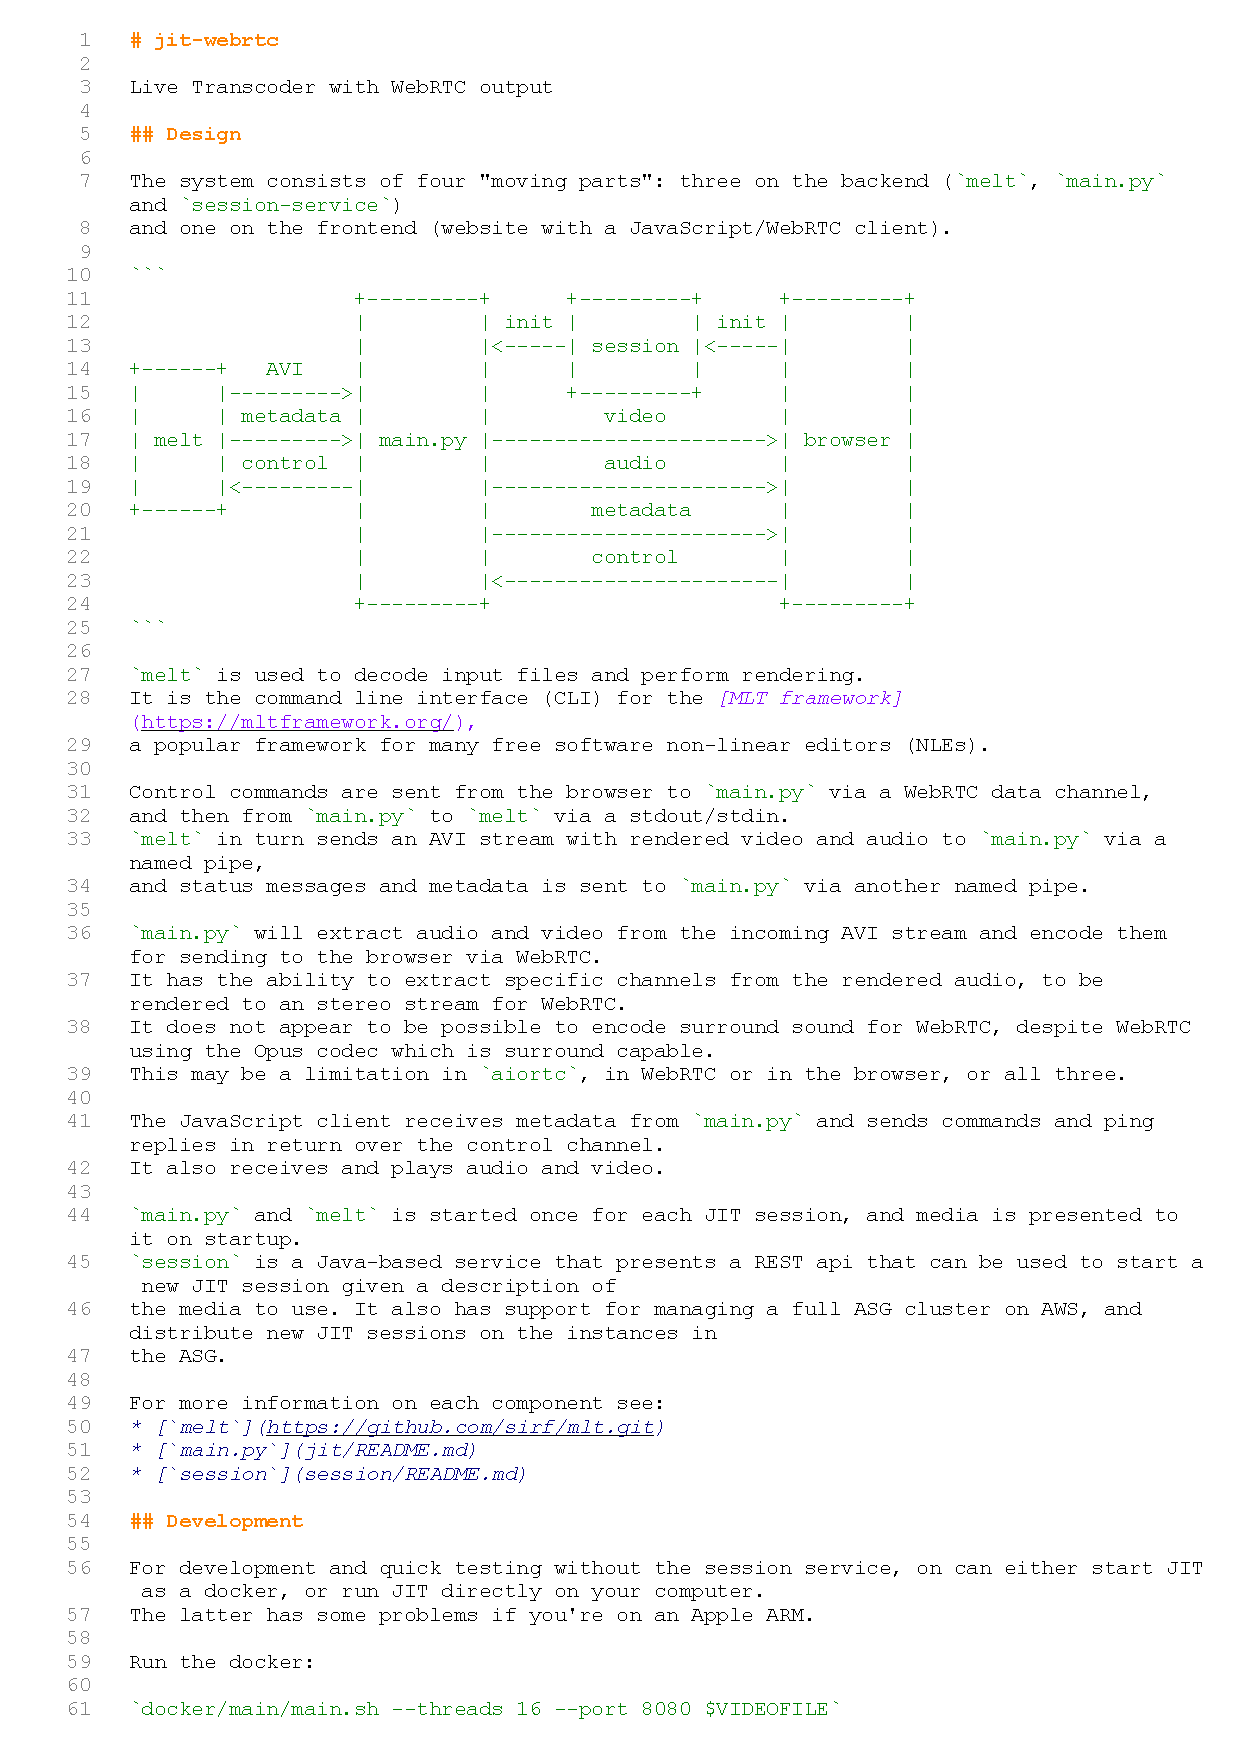
\includegraphics[page=1, width=0.9\textwidth]{BE.pdf}

\includegraphics[page=2, width=0.9\textwidth]{BE.pdf}




	


	
	
	
	
\end{document}